\documentclass[ a4paper, UKenglish, cleveref, autoref, thm-restate]{lipics-v2021}
\usepackage[utf8]{inputenc} % Required for inputting international characters
\usepackage[T1]{fontenc} % Output font encoding for international characters
% \usepackage[backend=bibtex,style=alphabetic,natbib=true]{biblatex}
% \usepackage[backend=bibtex,style=alphabetic,natbib=true]{biblatex}
% \addbibresource{references.bib}
\usepackage{amsmath, amssymb, amsfonts, amsthm, stmaryrd}
\usepackage{caption}
\usepackage{subcaption}
\usepackage{graphicx}
\usepackage{enumitem}
\usepackage{mathpartir}
\usepackage{bussproofs}
\usepackage{xparse}
\usepackage[usenames, dvipsnames]{xcolor}
\usepackage{lipsum}
\usepackage{xargs}
\usepackage{hyperref}
\usepackage{tikz-cd}
\usepackage{todonotes}
\usepackage{url}
\usepackage{xspace}
\usepackage{rotating}
\usepackage{quiver}
\usepackage{minted}
\usepackage{newunicodechar}
\usepackage{microtype}
% \addbibresource{references.bib}
\usepackage{array}   % for \newcolumntype macro
\newcolumntype{C}{>{$}c<{$}} % math-mode version of "l" column type
\newcolumntype{L}{>{$}l<{$}} % math-mode version of "l" column type

% \usepackage{draftwatermark}
% \SetWatermarkText{Confidential}
% \SetWatermarkScale{4}
% \SetWatermarkColor[gray]{0.9}

\hypersetup{
  linktocpage,
  colorlinks,
  citecolor=BlueViolet,
  filecolor=red,
  linkcolor=Blue,
  urlcolor=BrickRed
}
\newcommand{\mpav}[1]{\textcolor{red}{\textsc{Marco}: #1}}
\newcommand{\dcas}[1]{\textcolor{ForestGreen}{\textsc{David}: #1}}
\newcommand{\mvol}[1]{\textcolor{blue}{\textsc{Michael}: #1}}
\newcommand{\proofcomment}[1]{\text{\{ #1 \}}}
\newenvironment{proofof}[1] {\begin{proof}[Proof of {#1}]}{\end{proof}}
\newcommand{\eqdef}{\stackrel{\mathrm{\Delta}}{=}}
\newcommand{\eqiff}{\stackrel{\triangle}{\iff}}
\newcommand{\bnfeq}{\mathrel{::=}}
\newcommand{\defeq}{\triangleq}
\newcommand{\rul}[3]{\frac{#2}{#3}\;  {\textrulelabel{#1}}}
\newcommand{\den}[1]{\llbracket #1 \rrbracket}
\newcommand{\jud}[3]{#1 \vdash #2 : #3}
\newcommand{\bden}[1]{\llparenthesis#1 \rrparenthesis}
\newcommand{\bigslant}[2]{{\raisebox{.2em}{$#1$}\left/\raisebox{-.2em}{$#2$}\right.}}
\newcommand{\quotient}[2]{\bigslant{#1}{#2}}
\newcommand{\curry}{\Lambda}
\newcommand{\uncurry}{\begin{sideways}\begin{sideways}$\Lambda$\end{sideways}\end{sideways}}
\newcommand{\Bool}{\mathbb{B}}
\newcommand{\N}{\mathbb{N}}
\newcommand{\Nat}{\N}
\newcommand{\R}{\mathbb{R}}
\newcommand{\Sets}{\mathbf{Set}}
\newcommand{\blacklater}{\blacktriangleright}
\newcommand{\tot}{\mathcal{S}}
\newcommand{\PSh}{\ensuremath{\textbf{PSh}(\omega)}}

\newsavebox{\lbananabox}
\newcommand{\lbananamacro}{%
  
\begin{tikzpicture}[baseline=0.25em,xscale=0.005em,yscale=0.005em]
  \draw[solid, join=round] (2,0) to[out=140,in=-90] (0,3) to[out=90,in=-140] (2,6) -- (2.1,5.9)
              to[out=-120,in=90] (1.2,3) to[out=-90,in=120] (2.1,0.1) -- cycle;
\end{tikzpicture}
}
\savebox{\lbananabox}{\lbananamacro}
\newcommand{\lbanana}{\mathopen{\usebox{\lbananabox}\hspace{-0.6ex}}}


\newsavebox{\rbananabox}
\newcommand{\rbananamacro}{%
  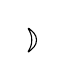
\begin{tikzpicture}[baseline=0.25em,xscale=-0.005em,yscale=0.005em]
  \draw[solid, join=round] (2,0) to[out=140,in=-90] (0,3) to[out=90,in=-140] (2,6) -- (2.1,5.9)
              to[out=-120,in=90] (1.2,3) to[out=-90,in=120] (2.1,0.1) -- cycle;
  \end{tikzpicture}
}
\savebox{\rbananabox}{\rbananamacro}
\newcommand{\rbanana}{\mathclose{\usebox{\rbananabox}}}


\newsavebox{\lbansbox}
\newcommand{\lbansmacro}{%
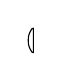
\begin{tikzpicture}[baseline=0.45ex,xscale=0.006em,yscale=0.012ex]%
% curvey bananas
%\draw[solid,join=round,fill=yellow] (2,0) to[out=140,in=-90] (0,3) to[out=90,in=-140] (2,6) -- (2.1,5.9) to[out=-120,in=90] (1.2,3) to[out=-90,in=120] (2.1,0.1) -- cycle;%
% fitted lenses
\draw[solid,join=round] (1.8,6) -- (1.5,5.9) to[out=-120, in=90] (0.7,3) to[out=-90, in=120] (1.5,0.1) -- (1.8,0) -- cycle;%
\end{tikzpicture}}
\savebox{\lbansbox}{\lbansmacro}
\newcommand{\lbans}{\mathopen{\usebox{\lbansbox}\mspace{1mu}}}

\newsavebox{\rbansbox}
\newcommand{\rbansmacro}{%
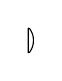
\begin{tikzpicture}[baseline=0.45ex,xscale=-0.006em,yscale=0.012ex]%
% curvey bananas
%\draw[solid,join=round,fill=yellow] (2,0) to[out=140,in=-90] (0,3) to[out=90,in=-140] (2,6) -- (2.1,5.9) to[out=-120,in=90] (1.2,3) to[out=-90,in=120] (2.1,0.1) -- cycle;%
% fitted lenses
\draw[solid,join=round] (1.8,6) -- (1.5,5.9) to[out=-120, in=90] (0.7,3) to[out=-90, in=120] (1.5,0.1) -- (1.8,0) -- cycle;%
\end{tikzpicture}}
\savebox{\rbansbox}{\rbansmacro}
\newcommand{\rbans}{\mathclose{\mspace{1mu}\usebox{\rbansbox}}}

\newsavebox{\llensbox}
\newcommand{\llensmacro}{%
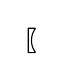
\begin{tikzpicture}[baseline=0.45ex,xscale=0.006em,yscale=0.012ex]%
\draw[solid,join=round] (1.4,0) -- (0,0) -- (0,6) -- (1.4,6) -- (1.5,5.9) to[out=-120, in=90] (0.7,3) to[out=-90, in=120] (1.5,0.1) -- cycle;%
\end{tikzpicture}}
\savebox{\llensbox}{\llensmacro}
\newcommand{\llens}{\mathopen{\usebox{\llensbox}\mspace{1mu}}}

\newsavebox{\rlensbox}
\newcommand{\rlensmacro}{%
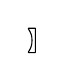
\begin{tikzpicture}[baseline=0.45ex,xscale=-0.006em,yscale=0.012ex]%
\draw[solid,join=round] (1.4,0) -- (0,0) -- (0,6) -- (1.4,6) -- (1.5,5.9) to[out=-120, in=90] (0.7,3) to[out=-90, in=120] (1.5,0.1) -- cycle;%
\end{tikzpicture}}
\savebox{\rlensbox}{\rlensmacro}
\newcommand{\rlens}{\mathclose{\mspace{1mu}\usebox{\rlensbox}}}

% filled versions
\newcommand{\Lbanana}{%
  \mathopen{\mspace{1mu}\tikz[baseline=0.25em,xscale=0.006em,yscale=0.006em]
  \fill (2,0) to[out=140,in=-90] (0,3) to[out=90,in=-140] (2,6) -- (2.1,5.9)
              to[out=-120,in=90] (1.2,3) to[out=-90,in=120] (2.1,0.1) -- cycle;\mspace{1mu}}}
\newcommand{\Rbanana}{%
  \mathclose{\mspace{1mu}\tikz[baseline=0.25em,xscale=-0.006em,yscale=0.006em]
  \fill (2,0) to[out=140,in=-90] (0,3) to[out=90,in=-140] (2,6) -- (2.1,5.9)
              to[out=-120,in=90] (1.2,3) to[out=-90,in=120] (2.1,0.1) -- cycle;}}
% % lens brackets (using TikZ)
% \newcommand{\llens}{%
%   \mathopen{\tikz[baseline=0.25em,xscale=0.006em,yscale=0.006em]
%   \draw[join=round] (1.4,0) -- (0,0) -- (0,6) -- (1.4,6) -- (1.5,5.9)
%         to[out=-120,in=90] (0.7,3) to[out=-90,in=120] (1.5,0.1) -- cycle;\mspace{1mu}}}
% \newcommand{\rlens}{%
%   \mathclose{\mspace{1mu}\tikz[baseline=0.25em,xscale=-0.006em,yscale=0.006em]
%   \draw[join=round] (1.4,0) -- (0,0) -- (0,6) -- (1.4,6) -- (1.5,5.9)
%         to[out=-120,in=90] (0.7,3) to[out=-90,in=120] (1.5,0.1) -- cycle;}}
% filled versions
\newcommand{\Llens}{%
  \mathopen{\tikz[baseline=0.25em,xscale=0.006em,yscale=0.006em]
  \fill (1.4,0) -- (0,0) -- (0,6) -- (1.4,6) -- (1.5,5.9)
        to[out=-120,in=90] (0.7,3) to[out=-90,in=120] (1.5,0.1) -- cycle;\mspace{1mu}}}
\newcommand{\Rlens}{%
  \mathclose{\mspace{1mu}\tikz[baseline=0.25em,xscale=-0.006em,yscale=0.006em]
  \fill (1.4,0) -- (0,0) -- (0,6) -- (1.4,6) -- (1.5,5.9)
        to[out=-120,in=90] (0.7,3) to[out=-90,in=120] (1.5,0.1) -- cycle;}}


\newcommand{\anamor}[1]{{\llens\, #1\, \rlens}}
\newcommand{\catamor}[1]{\lbans\, #1\, \rbans}
\newcommand{\cata}[1]{\lbans #1 \rbans}
\newcommand{\ana}[1]{\llens #1 \rlens}
\newcommand{\catafree}[1]{\Lbanana #1 \Rbanana}
\newcommand{\anacofree}[1]{\Llens #1 \Rlens}
\newcommand{\hylo}[2]{\cata{#1 \to #2}}
\newcommand{\cohylo}[2]{\ana{#1 \to #2}}
\newcommand{\fold}[1]{\catamor{#1}}
\newcommand{\unfold}[1]{\anamor{#1}}
\newcommand{\comp}{\cdot}
\newcommand{\operator}[1]{\textsf{#1}}
\newcommand{\head}{\operator{head}}
\newcommand{\inl}{\operator{inl}}
\newcommand{\inr}{\operator{inr}}
\newcommand{\tail}{\operator{tail}}
\newcommand{\Alg}{\text{-Alg}}
\newcommand{\Free}{\text{Free\xspace}}
\newcommand{\fmap}[1]{\text{fmap}\;#1}

\newcommand{\zero}{\operator{zero}}
\newcommand{\Nil}{\operator{nil}}
\newcommand{\Succ}{\operator{succ}}

\newcommand{\InOp}{\operator{in}^{\circ}}
\newcommand{\InIso}{\operator{in}}
\newcommand{\OutOp}{\operator{out}^{\circ}}
\newcommand{\OutIso}{\operator{out}}
\newcommand{\call}{\operator{call}}

\newcommand{\CatC}{\mathcal{C}}
\newcommand{\CatD}{\mathcal{D}}
\newcommand{\CatE}{\mathcal{E}}
\newcommand{\CatI}{\mathcal{I}}
\newcommand{\Set}{\mathbf{Set}}
\newcommand{\iso}{\cong}
\newcommand{\ceiling}[1]{\lceil #1 \rceil}
\newcommand{\floor}[1]{\lfloor #1 \rfloor}
\newcommand{\pair}[2]{\langle #1, #2 \rangle}
\newcommand{\haskell}[1]{\mintinline{haskell}{#1}}
%\newcommand{\coq}[1]{\mintinline{coq}{#1}}
\newmintinline[coq]{coq}{fontsize=\small}
\newmintinline[ocaml]{OCaml}{fontsize=\small}
\newminted{coq}{fontsize=\small}
\newminted{ocaml}{fontsize=\small}

\title{Magic-free Code Extraction of Generic Programs and Recursion Schemes in
Coq}

\bibliographystyle{plainurl}% the mandatory bibstyle
%\titlerunning{Dummy short title} %TODO optional, please use if title is longer than one line

\author{David Castro-Perez}{School of Computing, University of Kent}{d-castro-perez@kent.ac.uk}{}{}
\author{Marco Paviotti}{School of Computing, University of Kent}{m.paviotti@kent.ac.uk}{}{}
\author{Michael Vollmer}{School of Computing, University of Kent}{m.vollmer@kent.ac.uk}{}{}

%\author{Jane {Open Access}}{Dummy University Computing Laboratory, [optional: Address], Country \and My second affiliation, Country \and \url{http://www.myhomepage.edu} }{johnqpublic@dummyuni.org}{https://orcid.org/0000-0002-1825-0097}{(Optional) author-specific funding acknowledgements}%TODO mandatory, please use full name; only 1 author per \author macro; first two parameters are mandatory, other parameters can be empty. Please provide at least the name of the affiliation and the country. The full address is optional. Use additional curly braces to indicate the correct name splitting when the last name consists of multiple name parts.

%\author{Joan R. Public\footnote{Optional footnote, e.g. to mark corresponding author}}{Department of Informatics, Dummy College, [optional: Address], Country}{joanrpublic@dummycollege.org}{[orcid]}{[funding]}

\authorrunning{D. Castro-Perez, M. Paviotti, and M. Vollmer} %TODO mandatory. First: Use abbreviated first/middle names. Second (only in severe cases): Use first author plus 'et al.'

\Copyright{D. Castro-Perez, M. Paviotti, and M. Vollmer} %TODO mandatory, please use full first names. LIPIcs license is "CC-BY";  http://creativecommons.org/licenses/by/3.0/

\ccsdesc[100]{\textcolor{red}{Replace ccsdesc macro with valid one}} %TODO mandatory: Please choose ACM 2012 classifications from https://dl.acm.org/ccs/ccs_flat.cfm 

\keywords{hylomorphisms, Coq, code extraction, verification} %TODO mandatory; please add comma-separated list of keywords

\category{} %optional, e.g. invited paper

\relatedversion{} %optional, e.g. full version hosted on arXiv, HAL, or other respository/website
%\relatedversiondetails[linktext={opt. text shown instead of the URL}, cite=DBLP:books/mk/GrayR93]{Classification (e.g. Full Version, Extended Version, Previous Version}{URL to related version} %linktext and cite are optional

%\supplement{}%optional, e.g. related research data, source code, ... hosted on a repository like zenodo, figshare, GitHub, ...
%\supplementdetails[linktext={opt. text shown instead of the URL}, cite=DBLP:books/mk/GrayR93, subcategory={Description, Subcategory}, swhid={Software Heritage Identifier}]{General Classification (e.g. Software, Dataset, Model, ...)}{URL to related version} %linktext, cite, and subcategory are optional

%\funding{(Optional) general funding statement \dots}%optional, to capture a funding statement, which applies to all authors. Please enter author specific funding statements as fifth argument of the \author macro.

%\acknowledgements{I want to thank \dots}%optional

%\nolinenumbers %uncomment to disable line numbering



%Editor-only macros:: begin (do not touch as author)%%%%%%%%%%%%%%%%%%%%%%%%%%%%%%%%%%
\EventEditors{John Q. Open and Joan R. Access}
\EventNoEds{2}
\EventLongTitle{42nd Conference on Very Important Topics (CVIT 2016)}
\EventShortTitle{CVIT 2016}
\EventAcronym{CVIT}
\EventYear{2016}
\EventDate{December 24--27, 2016}
\EventLocation{Little Whinging, United Kingdom}
\EventLogo{}
\SeriesVolume{42}
\ArticleNo{23}
%%%%%%%%%%%%%%%%%%%%%%%%%%%%%%%%%%%%%%%%%%%%%%%%%%%%%%

\begin{document}

\maketitle

%TODO mandatory: add short abstract of the document
\begin{abstract}
  Generic programming with recursion schemes provides a powerful abstraction
  for reasoning about program equivalences and deriving optimisations which has
  been successfully applied to functional programming. However, formalising
  this technique in a type theory, (e.g. Coq) often requires compromises, such
  as imposing performance penalties, requiring the assumption of additional
  axioms, or introducing unsafe casts into extracted code (for example,
  \ocaml{Obj.magic} in OCaml).

  This paper presents a formalisation of hylomorphisms (a recursion scheme
  capturing divide-and-conquer algorithms) in Coq, along with their algebraic
  laws. The key contribution of this paper is that this formalisation is fully
  axiom-free, and it allows for the extraction of safe, idiomatic OCaml
  code for a variety of recursive programs. We formalise a series of divide-and
  conquer, dynamic programming, and mutual recursion programs and demonstrate
  that the extracted OCaml code for the programs formalised in our framework is
  efficient, resembles code that a human programmer would write, and contains
  no occurrences of \ocaml{Obj.magic}. We also present a machine-checked proof
  of the well-known short-cut fusion optimisation.
\end{abstract}

\section{Introduction}
\label{sec:intro}
Recursive definitions cannot be proven well-defined automatically due to the
halting problem. Modern proof assistants like Coq or Agda provide a sound, but
incomplete algorithm which syntactically checks for termination or
productivity.  For recursion, this is done by automatically inferring
which argument in the recursive call gets smaller with respects to the original
input argument.  For productivity, the algorithm checks that the corecursive
call appears directly under a constructor to make sure that this function
always produces at least one element after each recursive step.
This implies that some functions, though well-defined, cannot be accepted by
the proof assistant. Examples of this include common sorting algorithms, such
as quicksort and mergesort.
%One example is Quicksort, written in OCaml
%below:
\begin{minted}{OCaml}
let rec qsort xs = match divide xs with | None -> []
 | Some (pivot, (smaller, larger)) -> qsort smaller @ (pivot::qsort larger)
\end{minted}
While \ocaml{qsort} is a well-defined mathematical function it cannot be
accepted by a proof assistant.  The reason is that the \ocaml{divide}
function \emph{destructuring} the input ``dives'' deeper in the input returning
two sublists with the head as a pivot.

The main approach for implementing nonstructural recursion in Coq is to use
\emph{well-founded recursion}, where recursive definitions are coupled with
\emph{termination proofs}.  Using well-founded recursion, the recursive calls
will happen on \emph{structurally smaller termination proofs}\footnote{In Coq,
one approach is using the \coq{Fix} combinator, in which recursion is done on
an \emph{accesibility} predicate on the input, which is a proof that there are
no infinitely decreasing chains.}. A benefit of this approach is that,
extracting verified nonstructural recursive functions to OCaml will erase the
termination proofs, and so produce code that will be closer to what a
programmer may have written directly in OCaml. However, reasoning about program
equivalences requires dealing with such termination proofs, and it is common
practice to use custom reduction lemmas that will be used extensively when
proving properties about nonstructural recursive functions.

\emph{Structured recursion schemes} and their associated algebraic laws provide
an easier framework for reasoning about program equivalences.  In particular,
\ocaml{qsort} is an instance of a \emph{divide-and-conquer}
algorithm which, in the functional programming literature is known as a
hylomorphism~\cite{MeijerFP91, HuIT96}.  Hinze et al.~\cite{HinzeWG15} showed
that every recursive program (recursion scheme) can be formalised as a hylomorphism.
Furthermore, hylomorphism laws can capture a number of useful equivalences,
ranging from common optimisations such as \emph{short-cut
fusion}~\cite{TakanoM95}, to semi-automatic
parallelisations~\cite{Gibbons96:Third, farmsCastro}.

Not many approaches mechanise structured recursion
schemes in proof assistants.  Recently, Abreu et al.~\cite{AbreuDHJMS23} encode
an algebraic approach to divide-and-conquer computations, in which termination
is entirely enforced by the typing discipline of the recursion scheme. However,
although their approach solves the problem of termination proofs, as well as
the performance of the code that is run \emph{within Coq}, it no longer allows
the extraction of idiomatic OCaml code.  By this, we refer to code
that (1) does not preserve the recursive structure of common implementations;
and (2) lead to unsafe casts \ocaml{Obj.magic} in the generated code. 
In OCaml, \ocaml{Obj.magic} allows for unsafe casts between types.
Although the use of \ocaml{Obj.magic} should be safe in the code
extracted by Coq, it has been proven that, for higher-order programs, simple
interoperations can lead to incorrect behaviour or even
segfaults~\cite{forster:hal-04329663}. Therefore, the avoidance of axioms and
\ocaml{Obj.magic} means that the extracted code will have stronger
safety guarantees, and will allow the safe interoperation with other OCaml
code.

This work presents the first formalisation in Coq of \emph{hylomorphisms}, as
well as their algebraic laws that: (1) is \emph{axiom-free}; and (2)
allows the extraction of idiomatic OCaml code. While programmers
still need to reason about the termination of their programs, our mechanisation
will allow the use of the algebraic laws of hylomorphisms for program
reasoning, as well as extracting to idiomatic code. As an
example our mechanisation of \ocaml{qsort} as a hylomorphism will produce
the following code:
\begin{coqcode}
let rec qsort = function | [] -> []
  | h :: t -> let (l, r) = partition (fun x0 -> (<=) x0 h) t in
              let cx = fun p -> match p with | Lbranch -> l | Rbranch -> r in 
              app (qsort (cx Lbranch)) (h :: (qsort (cx Rbranch)))
\end{coqcode}
The contributions we make in this paper are as follows:
\begin{itemize}
  \item We provide a framework for \emph{generic programming} with recursion
    schemes in Coq, with a proof of their algebraic laws and 
    program equivalences, that allows clean code extraction.
  \item We formalise divide and conquer, dynamic programming, and
    mutual recursion algorithms.
  \item We verified the short-cut fusion optimisation in Coq and
    extract optimised code to OCaml.
\end{itemize}

% \section{Background on Recursion Schemes}
% Recursion schemes provide a systematic way to work with data types, such as
% trees or lists, by abstracting away the recursion into higher-order functions.
% Canonical recursion schemes include \emph{folds} (catamorphisms) which consume
% data and \emph{unfolds} (anamorphisms) which produce data. These are the unique
% solutions (when they exist) to the following two equations respectively
% \[
%   h  = a \comp F h \comp \InOp \qquad k = \OutOp \comp F k \comp c
% \]
% where $F$ is a \emph{base functor}, $Ff$ is the \emph{functorial action} which
% can be thought of the program $\operator{fmap}\; f$, $a$ is a program of type
% $F A \to A$ (an $F$-algebra),  $c$ is a program of type $C \to FC$ (a
% $F$-coalgebra), $\InOp$ is the isomoprhism on the least fixed-point of $F$,
% namely $\InOp : \mu F \to F\mu F$, and $\OutOp$ is the isomorphism on
% the greatest fixed-point of $F$, namely $F \nu F \to \nu F$. When
% the unique solutions to the above equations exist we denote them as $\cata{a}$
% and $\ana{c}$ respectively.

% \subsection{Hylomorphisms}
% Catamorphisms (dually anamorphisms) do not capture every recursion
% scheme we can think of.  As an example, consider an example of a classic
% \emph{divide-and-conquer} program such as quicksort algorithm:\footnote[1]{This
% program is written in Coq notation to be consistent, but it is not a program
% that Coq can accept.}

% \mpav{I need this to be written in Coq notation}
% \begin{coqcode}
% qs :: [a] -> [a]
% qs [] = []
% qs (x:xs) = qs (filter (x <=) xs) ++ [x] ++ (qs (filter (x >) xs))
% \end{coqcode}
% This program is formed of essentially two parts. The first one is what is
% commonly thought as the \emph{partition} function destructuring the input list
% in three parts, the pivot and the other two sublists, and the second part
% recursing over the sublists and composing the results back together.

% Notice that if we define the functor \coq{TreeF} $X = X \times A \times X$ with
% the obvious functorial action then \coq{partition} can be viewed as a
% \coq{TreeF}-coalgebra on lists over the type $A$
% \begin{coqcode}
% c : [A] -> TreeF [A]
% c (x:xs) = (filter (x <=) xs, x, filter (x >) xs)
% \end{coqcode}

% While we can define an \coq{TreeF}-algebra on lists
% over $A$ as well, that is a map
% \begin{coqcode}
% a : TreeF [A] -> [A]
% a (left, x, right) = left ++ [x] ++ right
% \end{coqcode}

% It should be easy to see that the program \coq{qs} can now be defined as the
% unique program that runs the coalgebra $c$ recurses over the sublists produced
% and then composes the results together. The structure exemplified by this
% program is a typical divide-and-conquer algorithm which can be implemented using
% an \emph{hylomorphism}. An hylomorphism is the unique solution $x : C \to A$ to
% the hylo equation
% \begin{equation}
%   \label{eq:hylo}
%   x =  a \comp Fx \comp c
% \end{equation}
% for a $F$-algebra on $A$, an $F$-coalgebra on $C$ and a functor $F$.  If for
% every $F$-algebra there exists a unique solution to (\ref{eq:hylo}) then we say
% the $F$-coalgebra $c$ is \emph{recursive}. Dually if for every $F$-coalgebra $c$
% there exists a unique solution to (\ref{eq:hylo}) we say the $F$-algebra $a$ is
% \emph{corecursive}. We denote the unique solution to the hylo equation
% (\ref{eq:hylo}) as $\hylo{a}{c}$.

% Moreover, it shoud be easy to see that catamorphisms and anamorphism arise as a
% special case of hylomorphisms
% \begin{equation}
%   \label{eq:cata}
%   \cata{a} = \hylo{\InOp}{a} \qquad \ana{c} = \hylo{c}{\OutOp}
% \end{equation}
% since $\InOp$ is indeed a recursive coalgebra and $\OutOp$ is a corecursive
% algebra.

% \subsection{Implementing Recursion Schemes}
% Hylomorphisms can implement all structured recursion schemes~\cite{HinzeWG15,
% HinzeW16}.  Here we show the result by means of a very basic example: mutual
% recursion. We refer the reader to Hinze et al.~\cite{HinzeWG15} for the
% theoretical result and to Yang and Wu~\cite{YangW22} for more examples of
% recursion schemes.

% % More specifically, in the context of recursive data types, such as in Haskell,
% % where induction and coinduction is conflated, an hylomorphism can be implemented
% % in terms of a catarmorphism (folding) and an anamorphism (unfolding)
% % \[
% %   \hylo{a}{c} = \cata{a} \comp \ana{c}
% % \]
% % They first generate a data structure using an anamorphism and then immediately
% % fold or reduce it using a catamorphism.

% % The hylomorphism pattern is particularly useful for defining recursive
% % algorithms in a functional programming context, where recursion is a fundamental
% % tool for solving problems. By separating the generation of data structures from
% % their consumption, hylomorphisms enable clearer and more modular code, making it
% % easier to reason about and maintain recursive algorithms.

% % However, in a type theory inductive and coinductive data types are separate.

% % In this section we will introduce the notion of hylomorphism. By way of examples
% % we will also give high level intution as to way all recursion schemes can be
% % defined in terms of a basic

% Say that we want to prove that the two mutually recursive functions below are
% well-defined

% \begin{tabular}{LL}
%   \operator{even} : \Nat \to \Bool                  &  \operator{odd} : \Nat \to \Bool\\
%   \operator{even} (0) = \top                        &  \operator{odd}(0) = \bot\\
%   \operator{even} (n+1) = \neg \operator{odd}(n)    &  \operator{odd}(n+1) = \neg (\operator{even}(n))
% \end{tabular}

% One option is to prove that the following function is
% equivalent to the above
% \begin{align*}
%   & \operator{even-odd} : \Nat \to \Bool \times \Bool\\
%   & \operator{even-odd} (0) = (\top, \bot)\\
%   & \operator{even-odd} (n+1) = \operator{let } (x,y) \leftarrow \operator{even-odd}(n) \operator{ in } (\neg x, \neg y)
% \end{align*}
% which is clearly a catamorphism $\cata{a}$ with $a (\Nil) = (\top, \bot)$ and
% $a(\operator{x,y}) = (\neg x, \neg y)$ and hence an hylomorphism as defined in
% (\ref{eq:cata}).  Now we are left to show they are equivalent. Well, it is easy
% to do so since $\operator{even} = \pi_{1} \comp \operator{even-odd}$
% $\operator{odd} = \pi_{2} \comp \operator{even-odd}$. The proof that these two
% pairs of functions are the same is an easy induction over the natural numbers.

% This is an instance of a more general phenonema whose argument uses the concept
% of an adjunction~\cite{MacLane71}.  For this particular example, the argument is
% as follows.  There is an isomorphism between pairs of maps
% $(A \to B_{1}, A \to B_{2})$ and maps $(A \to B_{1} \times B_{2})$.  This is
% given by $\Phi (f,g) = \pair{f}{g}$ and
% $\Psi(f) = (\pi_{1} \comp f, \pi_{2} \comp f)$ where the projections $\pi$ are
% part of the counit of the adjunction between the diagonal functor
% $\Delta X = (X,X)$ and the product $\times$.  Once this correspondence is
% established we can implement the map $A \to B_{1} \times B_{2}$ as an
% hylomorphism and derive the original and more complex recursion scheme.

% % In general an adjunction is a natural correspondence of maps
% % \[
% %   LA \to B \iff A \to RB
% % \]
% % where $L$ and $R$ are called adjoints.

% However, formalising adjunctions in Coq would require to formalise a
% non-negligible amount of category theory which goes beyond the scope of the
% present work. In this paper, we will instead derive the recursion schemes as
% needed and implement them as hylos.
% % \subsubsection{Course-of-Value Recursion}
% % The knapsack algorithm is defined as following in pseudo-Haskell code:
% % \begin{align*}
% %   & \operator{knapsack} : [(\Nat, \R)] \to \Nat \to \R\\
% %   & \operator{knapsack}\;wvs\; c = \operator{maximum}_{0}
% %     [v + \operator{knapsack}\;wvs\; (c - w) \mid (w,v) \leftarrow wvs, w \le c]
% % \end{align*}
% % %
% % with dynamic programming knapsack can be rephrased like this
% % \begin{align*}
% %   & \operator{knapsack} : [(\Nat, \R)] \to \Nat \to \R\\
% %   & \operator{knapsack}\;wvs\;c= table !! c \\
% %   & \qquad table  = [ks\;i \mid i \leftarrow [0..c]]\\
% %   & \qquad ks\; i = maximum_{0} [v + table!! (i - w) \mid (w,v) \leftarrow wvs, w \le i]
% % \end{align*}

% % The recursion scheme is justified by solving a recursive equation.  First we
% % define an operation to create a memory table representing the list of capacities
% % $[0..c]$. We first define a functor $D X = 1 + X$ representing the base functor
% % for constructing the naturals $\Nat = \mu D$ the we define the generating
% % function by induction on the naturals
% % \begin{align*}
% %   & \operator{fan} : \Nat \to D_{\infty}\Nat\\
% %   & \operator{fan} (0)    = \pair{0}{\inl}\\
% %   & \operator{fan} (n+1)  = \pair{n+1}{\inr (\operator{fan}(n))}
% % \end{align*}
% % The recursion scheme from a comonad is then defined as follows
% % \begin{align*}
% %   & \operator{rsfc} : \Nat \to A\\
% %   & \operator{rsfc} = alg \comp DD_{\infty}(\operator{rsfc}) \comp D(\operator{fan}) \comp \InOp
% % \end{align*}
% % At his point we can given the definition of the algebra $alg$ which effectively implements knapsack.
% % Firs we define the $\operator{lookup}$ function which returns (if present) the element indexed in the memory table
% % \begin{align*}
% %   & \operator{lookup} : \Nat \to D_{\infty} \R \to \R_{\bot}\\
% %   & \operator{lookup} (0,   \pair{r}{\textunderscore})  = r\\
% %   & \operator{lookup} (n+1, \pair{r}{\inl})         = \bot\\
% %   & \operator{lookup} (n+1, \pair{r}{\inr(table)})  = \operator{lookup} (n, table)
% % \end{align*}
% % and now we can define the algebra over the reals
% % \begin{align*}
% %   & \operator{alg} : DD_{\infty} \R \to \R\\
% %   & \operator{alg}\; (\inl)  = 0\\
% %   & \operator{alg}\; (\inr(table))  = \operator{maximun}_{0} [ v + \operator{lookup}\; table\; (i - w) \mid (w,v) \leftarrow wvs, w \le i]
% % \end{align*}

% % It remains to show how an $\operator{rsfc}$ is implemented in terms of
% % hylomorhisms.

% % \paragraph{Implementation into hylomorphisms}
% % In order to implement rsfcs as hylos we need a parametric distributive law
% % \[
% %   \lambda_{X} : GG_{\infty}X \to G_{\infty}GX
% % \]
% % This can be defined as
% % $\lambda = G_{\infty}G(\head) \comp \anacofree{G(\tail)}$.  The distributive law
% % is instrumental to be able to lift coalgebras in the following sense. Give a
% % $G$-coalgebra on $X$, a lifting $H$ is a functor which lifts this coalgebra to a
% % $G$-coalgebra on $HX$.  In particular, the lifting $G_{\lambda}$ takes
% % $G_{\infty}$-coalgebras on $X$ and transforms them into $G_{\infty}$-coalgebras
% % on $GX$
% % \begin{align*}
% %   & G_{\lambda}(c) : GA \to G_{\infty} GA\\
% %   & G_{\lambda}(c) = \lambda \comp G (c)
% % \end{align*}
% % where $c : C \to GC$.

% % Now, given an algebra $a : GG_{\infty} A \to A$ on the carrier $A$ we can
% % convert it into an algebra for the carrier $G_{\infty} A$ by
% % \begin{align*}
% %   & \floor{a} : GG_{\infty} A \to G_{\infty} A\\
% %   & \floor{a} = G_{\infty}(a) \comp \anacofree{G_{\lambda}(\delta)}
% % \end{align*}
% % where $\eta_{A} : A \to G_{\infty} A$ is the unit of the comonad creating an
% % infinite constant list.

% % At this point the hylo is simply defined by
% % $\hylo{\InOp}{a} : \mu F \to G_{\infty}A$  and the rsfc is derived as follows
% % \begin{align*}
% %   & \operator{rsfc} : \mu G \to A \\
% %   & \operator{rsfc} = \head \comp \hylo{\InOp}{a}
% % \end{align*}

% % % \subsection{Catamorphisms and Anamorphism}
% % % A catamorphism is the unique program defined as
% % % \[
% % %   x = a \comp \fmap{x} \comp \InOp
% % % \]
% % % Can be implemented:
% % % \[
% % %   \cata{a} = \hylo{\InOp}{a}
% % % \]

% % % An anamorphism is the unique program satisfying the equation
% % % \[
% % %   x = \OutOp \comp \fmap{x} \comp{c}
% % % \]
% % % The anamorphism is indicated by $\ana{c}$. Recursion schemes given by a
% % % corecursive algebra such as $\OutIso$ are also called hylomorphism but they are
% % % indicated with the symbol for the anamorphism, $\cohylo{c}{\OutOp}$.

% % \paragraph{Free Monads}
% % Given an endofunctor $D$ and a type $A$ the free monad is defined as the least
% % solution to the following domain equation
% % \[
% %   D^{*}A = A + DD^{*}A
% % \]
% % where $\eta_{A} : A \to D^{*}A$ is the left injection and
% % $\call_{A} : DD^{*}A \to D^{*}A$ is the right injection. Given an algebra
% % $a : DA \to A$ there is a unique solution to the following recursive equation
% % \[
% %   x \comp \call_{A} = a \comp D(x)
% % \]
% % that is $\catafree{a} = \cata{[id_{A}; a]}$. With this operation we can extend
% % the free algebra $\call$ to the multiplication $\mu : D^{*}D^{*}A \to D^{*}A$
% % defined as $\mu = \catafree{\call}$.

% % \paragraph{Cofree Comonads}
% % Given an endofunctor $D$ and a type $A$ the cofree comonad is defined as the
% % greatest solution to the following domain equation
% % \[
% %   D_{\infty}A = A + DD_{\infty}A
% % \]
% % where $\head : D_{\infty}A \to A$ is the first projection and
% % $\tail_{A} : D_{\infty}A \to DD_{\infty}A$ is the second projection.
% % Given an algebra $c : A \to DA$ there is a unique solution to the following
% % recursive equation
% % \[
% %   \tail_{A} \comp x = D(x) \comp c
% % \]
% % that is $\anacofree{c} = \ana{\pair{id_{A}}{c}}$. With the latter operation we
% % can extend $\tail$ to the comultiplication for the comonad
% % $\delta : D_{\infty}A \to D_{\infty} D_{\infty}A$ defined by
% % $\delta = \anacofree{\tail}$.


% % \subsection{Accumulators}
% % For an algebra $a : D(A^{P})\times P \to A$:
% % \begin{align*}
% %   & g : \mu D \times P \to B\\
% %   & g (d, p) = a (\fmap{(\curry g)} \comp \InOp(d), p)
% % \end{align*}

% % \paragraph{Hylo Implementation}
% % Given an algebra $a : D(A^{P}) \to A^{P}$ the accumorphism corresponds to the unique
% % solution to the following equation
% % \begin{align*}
% %   & f : \mu D \to A^{P}\\
% %   & f = a \comp \fmap (f) \comp \InOp
% % \end{align*}
% % thus $f = \hylo{\InOp}{a}$.

% % The complex recursion scheme is then
% % $g = \uncurry\hylo{\InOp}{a} : \mu D \times P \to B$.

% % \subsection{Mutu-Hylo}
% % For an algebra $a_{1} : D(A_{1} \times A_{2}) \to A_{1}$ and an algebra
% % $a_{2} : D(A_{1} \times A_{2}) \to A_{2}$:
% % \begin{align*}
% %   & (g_{1}, g_{2}) : (\mu D, \mu D) \to (A_{1}, A_{2})\\
% %   & (g_{1}, g_{2}) = (a_{1}, a_{2}) \comp (\fmap{\pair{g_{1}}{g_{2}}},\fmap{\pair{g_{1}}{g_{2}}}) \comp (\InOp, \InOp)
% % \end{align*}

% % \paragraph{Hylo Implementation}
% % Given an algebra $a : D(A_{1} \times A_{2}) \to A_{1} \times A_{2}$
% % \begin{align*}
% %   & f : \mu D \to A_{1} \times A_{2}\\
% %   & f = a \comp \fmap{f} \comp \InOp
% % \end{align*}
% % for which the solution is an hylo $f = \hylo{\InOp}{a}$.

% % The mutumorphism can be implemented as
% % $(g_{1}, g_{2}) = (\pi_{1} \comp f, \pi_{2} \comp f)$.

% % \paragraph{Coq Implementation}
% % Given the two algebras  $a_{1} : D(A_{1} \times A_{2}) \to A_{1}$ and
% % $a_{2} : D(A_{1} \times A_{2}) \to A_{2}$.
% % We define the two recursive functions  $f_{1}$ and $f_{2}$ as

% % \[
% %   f_{1} = \pi_{1} \comp \hylo{\InIso}{\pair{a_{1}}{a_{2}}} \qquad f_{2} = \pi_{2} \comp \hylo{\InIso}{\pair{a_{1}}{a_{2}}}
% % \]
% % % A recursion scheme from a comonad $D_{\infty}$ for a data functor $F$

% % % For example, for the functor $(1 + -)$ an algebra over this functor is a
% % % function $1 + X \to X$ is a pair of functions $\Nil : 1 \to X$ and
% % % $\Succ : X \to X$. The cofree comonad over $D$ is defined as follows
% % % \[
% % %   D_{\infty} A \iso A \times (1 + D_{\infty})
% % % \]
% % % which is the the type of non-empty possibly infinite lists with elements in $A$


% % % First we have to assume a distributive law
% % % $\lambda : DD_{\infty} \to D_{\infty}D$.  For an algebra
% % % $a : D(D_{\infty} A) \to A$,
% % % \begin{align*}
% % %   & g : \mu D \to A\\
% % %   & g = a \comp D(G_{\infty}(g) \comp \anacofree{\cata{G^{\lambda}(\InIso)}}) \comp \InOp
% % % \end{align*}
% % % where
% % % $G^{\lambda} (alg : D\mu F \to \mu F) = DGX \xrightarrow{\lambda} GDX \xrightarrow{G(alg)} GX$
% % % is a $D$-algebra on $GX$. The catamorphism of this algebra has the following
% % % type
% % % \[
% % %   \cata{G^{\lambda}(\InIso)} : \mu D \to G\mu D
% % % \]
% % % which is the type of a $G$-algebra used to initialise the memory table.

% % % Given an algebra $a : DG_{\infty} A \to G_{\infty} A$ we can equivalently ask
% % % what is the unique solution of the following equation
% % % \begin{align*}
% % %   & f : \mu F \to G_{\infty} A\\
% % %   & f = a \comp \fmap{f} \comp \InOp
% % % \end{align*}
% % % The solution to this equation can be found again using an hylo
% % % $f = \hylo{\InOp}{a} : \mu F \to G_{\infty} A$.  The course-of-value recursion
% % % can be recovered from this by setting $g = \head \comp f$

% % % \subsubsection{Histomorphism}

% % % The definition of $\lambda$ is:
% % % \begin{align*}
% % %   & \lambda : GG_{\infty} A \to G_{\infty} GA\\
% % %   & \lambda = \fmap{(\fmap{\head})}\comp \anacofree{\fmap{\tail}}
% % % \end{align*}
% % % For example, for $GX = 1 + X$ we have to define
% % % \begin{align*}
% % %   & \lambda : 1 + G_{\infty} A \to G_{\infty} (1 + A)\\
% % %   & \lambda(\inl) = \pair{\inl}{\lambda(\inl)}\\
% % %   & \lambda(\inr(table)) = \pair{\inr (\head(table))}{\lambda (\tail (table))}
% % % \end{align*}

% % % % \begin{align*}
% % % %   & \operator{lookup} :: \Nat \to G_{\infty} \R \to \operator{Maybe}\;\R\\
% % % %   & \operator{lookup}\; \Zero       (\Cons{a}{\text{\textunderscore}})     = \Just{a}\\
% % % %   & \operator{lookup}\; (\Succ{n})  (\Cons{a}{\Zero})                      = \Nothing\\
% % % %   & \operator{lookup}\; (\Succ{n})  (\Cons{a}{\Succ table})                = \operator{lookup}\; n  table
% % % % \end{align*}

% % % % Defining the algebra
% % % % \begin{align*}
% % % %   & \operator{alg} :: D (G_{\infty} \R) \to \R\\
% % % %   & \operator{alg}\; Zero           = 0\\
% % % %   & \operator{alg}\; (Succ{table}) = maximum_{0} [v + \operator{lookup}\; table (i - w) | (w,v) \leftarrow wvs, w \le i]
% % % % \end{align*}

\section{Mechanising Extractable Container Functors}
In order to abstract recursion patters we need to be able to abstract away from
the particular shape of the data.  This is achieved by introducing the concept
of \emph{functors} which have the suitable fixed-point properties, i.e.\ those
who have a initial algebras. A common approach to construct such functors is to
use \emph{containers}~\cite{AbbottAG05} (Section~\ref{sec:containers}).
However, reasoning about container equality
will require us to consider both functional extensionality and heterogeneous
equality. We avoid these axioms by introducing a
custom equivalence relation on types (Section~\ref{sec:types-morphisms}).

\subsection{Functors and Containers}
\label{sec:containers}
Functors are functions \coq{F : Type -> Type} which additionally have a
map \coq{fmap : forall A B, (A -> B) -> F A -> F B} witnessing the idea that a
functor represents a container for abstract data that can be manipulated without
changing the outer structure. For example, the type \coq{List : Type -> Type} is
a functor and \coq{List A} is the type of lists over elements of type \coq{A}
with the obvious \coq{fmap} function recursively traversing a list and applying
the function \coq{A -> B} for each element. Additionally, the type of
lists \coq{List A} arises as the least fixed-point of the
functor \coq{F X = unit + (A * X) }.

In general not every functor has a fixed-point, and it is not possible to build
the fixed-point of a functor such as \coq{F} in Coq due to not being strictly
positive.  Due to this, we are going to restrict to \emph{polynomial functors}
as represented by containers.  A container is defined by a type of
\emph{shapes} and a \emph{family of position types} indexed by shapes.
\begin{coqcode}
Context (Shape : Type) (Pos : Shape -> Type).
\end{coqcode}
For the functor \coq{F} we introduced in the previous paragraph we would define
\coq{Shape} as \coq{unit + A} indicating there are two constructors in the data
type and one of these contains a piece of data of type \coq{A}.  Moreover, we
would define the positions as \coq{Pos (inl tt) = Empty_set} and 
\coq{Pos (inr a) = unit} indicating that the first constructor does not have
any type variables and the second constructor has one type variable.

At this point an \emph{extension} of this container is a functor defined as
follows:
\begin{coqcode}
Record App (X : Type) := MkApp { shape : Shape; contents : Pos shape -> X }.
\end{coqcode}
with the obvious action on morphisms given by post-composition
with \coq{contents}.
\begin{coqcode}
Definition fmap (f : A -> B) (x : App C A) : App C B
  := {| shape := shape x; contents := fun e => f (contents x e) |}
\end{coqcode}
In our running example, the type \coq{App X}, for
some \coq{X} has two inhabitants.  The first is a pair composed
by \coq{inl tt : Shape} and a function \coq{Pos (inl tt) -> X}. This latter is
in fact a function of type \coq{Empty_set -> X}. This pair is, therefore
isomorphic to the type \coq{unit}, the type with only one inhabitant.  The
second inhabitant is the pair composed by \coq{inr a : Shape}, for
some \coq{a : A}, and a function \coq{Pos (inr a) -> X}.  This latter type is
equal to \coq{unit -> X} which represents the elements of \coq{X} and therefore
is isomorphic to \coq{X}.  This particular pair of shapes and positions is 
therefore isomorphic to the type \coq{unit + A * X}.

The correspondence between containers and polynomial functors has been
formalised in this work and can be found in the accompanying code (file
Container.v). 
% 
%Generally, any functor that
%is isomorphic to a container extension is called a \emph{container functor}.
%Here we will call \emph{container functor} the functors defined by a specific
%container extension.

\subsection{Extractable Containers}
In the previous section we defined containers using dependent types.  However,
Ocaml's type system is not equipped to handle these. To solve this problem
Coq's code extraction mechanism will insert unsafe casts.

Consider instead representing the positions of a container using a decidable
validity predicate (\coq{valid}) which assigns shapes to positions. We use
boolean functions and coercions from \coq{bool} to \coq{Prop} to represent
decidable predicates, similarly to SSReflect~\cite{GonthierL09}. The family of
positions for a given shape in a container can be recovered by defining:
\begin{coqcode}
Class Cont (Shape : Type) (APos : Type) := { valid : Shape -> APos -> bool }.
Record Pos `(C : Cont Shape APos) (shape : Shape) :=
  ValidPos { val : APos; IsValid : valid shape pos }.
\end{coqcode}
Coq's code extraction will now be able to erase the validity predicate, and
generate OCaml code that is free of unsafe casts. The OCaml code extracted for
\coq{Pos} will now be exactly the code extracted for \coq{APos}.
The decidability of the validity predicate is crucial for our purposes of 
remaining axiom-free. To illustrate this, suppose that we need to show
the equality of two container extensions. We will need to show that, for
the same positions, they will produce the same result. In Coq, the goal
would look as follows: 
\begin{coqcode}
 k : Pos C s -> X
 P1, P2 : valid s p
 ---------------------------
 k (ValidPos p P1) = k (ValidPos p P2)
\end{coqcode}
If \coq{valid} was a regular proposition in \coq{Prop}, it would not possible
to prove the equality of \coq{P1} and \coq{P2}. However, by using a decidable
predicate, if we know that \coq{P1} and \coq{P2} are of type 
\coq{valid s p = true}, then we can prove without any axioms that 
\coq{P1 = P2 = eq_refl}.


% A container extension is then defined as follows:
% \begin{coqcode}
% Context (Shape : Type) (Pos : Type) (Valid : Shape -> Pos -> Prop).
% Record App (X : Type) := { shape    : Shape;
%                           contents : {p | Valid shape p} -> X }.
% \end{coqcode}
% This approach solves the problem of the unsafe casts, since the code extracted
% for \coq{{p | Valid shape pos}} will be an OCaml singleton type defined as the
% OCaml equivalent to \coq{Pos}.

\subsubsection{Equality of Container Extensions}
Reasoning about the equality of container extensions is not entirely solved by
using decidable validity predicates to define the families of positions. In
general, we want to equate container extensions that have the same shape, and
that, for equal shape and position, they return the same element. To avoid the
use of the functional extensionality axiom, we capture this relation with the
following inductive proposition in Coq:
\begin{coqcode}
Inductive AppR `{F : Cont Sh P} {X} (x y : App F X) : Prop :=
| AppR_ext (Es : shape x = shape y)
           (Ek : forall e1 e2, val e1 = val e2 -> cont x e1 = cont y e2).
\end{coqcode}
Note that  we do not care about the validity proof of the positions, only their
value. This is to simplify (slightly) our proofs. This relation is
trivially \emph{reflexive}, \emph{transitive}, and \emph{symmetric}.

However, the use of a different equality for container extensions now forces us
to deal with the fact that some types have different definitions of equality.
In particular, we want to reason about the equality of functions of types such
as \coq{App F A -> B} (or \coq{B -> App F A}). Since 
these types now come with their own equivalence, any function that manipulates
them needs to be \emph{respectful}. I.e.\ given 
\coq{R : X -> X -> Prop} and \coq{R' : Y -> Y -> Prop},
we want functions (morphisms) that satisfy the following property:
\begin{coqcode}
forall (x y : X), R x y -> R' (f x) (f y)
\end{coqcode}

\subsection{Types and Morphisms}
\label{sec:types-morphisms}
We address the different forms of equality by defining a class of
\emph{setoids}, types with an associated equivalence relation, and considering
only functions that respect the associated equivalences, or \emph{proper}
morphisms with respect to the function \emph{respectfulness} relation. We use
the type-class mechanism, instead of setoids in Coq's standard library, to help
Coq's code extraction mechanism remove any occurence of custom equivalence
relations in the extracted OCaml code. We use \coq{=e} to denote the equivalence
relation of a setoid. By default, we associate every Coq type with the standard
propositional equality, unless a different equivalence is specified (we allow
overlapping instances, and Coq's propositional equality takes the lowest
priority).
%\begin{coqcode}
%Reserved Notation "f =e g" (at level 70, no associativity).
%Class setoid A : Type :=
%  MkEquiv
%    { eqRel : A -> A -> Prop;
%      e_refl : forall x, eqRel x x;
%      e_sym : forall x y, eqRel x y -> eqRel y x;
%      e_trans : forall x y z, eqRel x y -> eqRel y z -> eqRel x z;
%    }.
%Notation "f =e g" := (eqRel f g).
%\end{coqcode}
Given types \coq{A} and  \coq{B}, with their respective
equivalence relations \coq{eA : A -> A -> Prop} and
\coq{eB : B -> B -> Prop}, the we define the type
\coq{A ~> B} to represent \emph{proper} morphisms of the
respectfulness relation of \coq{R} to \coq{R'}.
\begin{coqcode}
Structure morph A {eA : setoid A} B {eB : setoid B} :=
  MkMorph { app :> A -> B; app_eq : forall x y, x =e y -> app x =e app y }.
Notation "A ~> B" := (@morph A _ B _).
\end{coqcode}
We rely on Coq's type class mechanism to fill in the necessary equivalence
relations. Coq's code extraction mechanism will erase any occurrence
of \coq{Prop} in the code, so objects of type \coq{A ~> B} will be extracted to
the OCaml equivalent to \coq{A -> B}. Note the implicit coercion
from \coq{A ~> B} to \coq{A -> B}.
On top of this, we define basic function composition and identity functions:
\begin{coqcode}
Notation "f \o g" = (comp f g).
Definition comp : (B ~> C) ~> (A ~> B) ~> A ~> C := ...
Definition id : A ~> A := ...
\end{coqcode}
Using custom equivalences and proper morphisms, we redefine the definitions of
container extensions and container equality. In particular, container
extensions require a proper morphism to check the validity of positions in
shapes, and container equality now uses equivalences of shapes and contained
elements: 
\begin{coqcode}
Class Cont `{setoid Shape} (Pos : Type) := { valid : Shape * Pos ~> bool }.
Inductive AppR `{F : Cont Sf Pf} `{setoid X} (x y : App F X) : Prop :=
  | AppR_ext (Es : shape x =e shape y)
             (Ek : forall e1 e2, val e1 = val e2 -> cont x e1 =e cont y e2).
\end{coqcode}
Note the use of \coq{=e} instead of Coq's standard equality.  For positions,
however, we chose to use Coq's propositional equality, since these would leads
to simpler code. We explain why in Section~\ref{sec:algebras}, and the
mechanisation of initial algebras of container extensions.
%The definitions in
%Figure~\ref{fig:poly} are redefined to account for these changes in a
%straightforward way, i.e. we prove that validity predicates are indeed proper
%morphisms. 

This definition leads to the well-known ``setoid hell'', which we mitigate by
providing tactics and notations to automatically discharge proofs of
\coq{app_eq} for morphisms, whenever the types use the standard propositional
equality, or a combination of propositional and extensional equality. However,
our compositional approach allows us to build morphisms by plugging in other
morphisms to our combinators. In our framework, our expectation is that the
user-provided functions remain small, with relatively straightforward proofs of
\coq{app_eq}.

However, by using this mechanisation, we gain simplified proofs via the use of
Coq's \emph{Generalised Rewriting}. Since every morphism \coq{f : A ~> B}
satisfies the property that if \coq{x =e y}, then \coq{f x =e f y}, we can add
every morphism as a proper element of Coq's respectfulness relation. In
practice, this means that we can use the \coq{rewrite} tactic on proofs of
type \coq{A =e B}, for arbitrary \coq{A} and \coq{B}, whenever they are used as
arguments of morphisms, as well as Coq's \coq{reflexivity}, \coq{symmmetry},
and \coq{transitivity} tactics. For example:
\begin{coqcode}
Goal forall `(f : A ~> B) `(g : B ~> C) `(h : C ~> D) (H : h \o g =e id), 
  h \o (g \o f) =e f.
Proof.  rewrite compA, H.  reflexivity. Qed.
\end{coqcode}

\subsubsection{Polynomial Types}
We define a number of equivalences for polynomial types.
%These equivalences are
%be used when building proper morphisms that manipulate their respective types.
\begin{coqcode}
Instance ext_eq (A : Type) `{eq_B : setoid B} : setoid (A -> B).
Instance pair_eq `{eq_A : setoid A} `{eq_B : setoid B} : setoid (A * B).
Instance sum_eq `{eq_A : setoid A} `{eq_B : setoid B} : setoid (A + B).
Instance prop_eq : setoid Prop.
Instance pred_sub `{eA : setoid A} {P : A -> Prop} : setoid {a : A | P a}.
\end{coqcode}
Most of the definitions that involve functions and polynomial types are
straightworward.  Identity and composition are defined as 
\coq{fun x => x} and \coq{fun f g x => f (g x)} 
respectively, and the proofs that they are proper morphisms is straightforward,
and automatically discharged by Coq. 
Products are built using function \coq{fun f g x => (f x, g x)},
with the projections being the standard Coq  \coq{fst} and
\coq{snd} functions. Similarly, sum injections are encoded using
Coq's \coq{inl} and \coq{inr} constructors, and
pattern matching on them uses the function 
\coq{fun f g x => match x with | inl y => f y | inr y => g y end}.
The proofs that these morphisms are proper are straightforward.  Finally, we
also provide functions for currying/uncurrying, and  flipping the arguments of
a proper morphism. We force most of our definitions to be inlined, to help
Coq's code extraction mechanism to inline as many of these combinators as
possible.

We prove the isomorphisms of polynomial types and the equivalent 
container extensions. As an example, we discuss (informally) the isomorphisms
of pairs with their equivalent container extensions. Suppose that we
know that \coq{App F X} is isomorphic to \coq{A}, and
\coq{App G X} is isomorphic to \coq{B}. Then we can
show that \coq{App (Prod F G) X} is isomorphic to
\coq{A * B}.  If we have an element of type 
\coq{App (Prod F G) X},
using the \coq{inl} position, we can obtain
\coq{App F X}.  Similarly, using \coq{inr}, we can
obtain \coq{App G X}. Since these are the only two valid positions
in the shape of pairs, we have finished. It is now sufficient to use the
isomorphisms of \coq{App F X} and \coq{App G X} to
obtain \coq{A * B}. Similarly if we have \coq{A * B},
we can first use the isomorphisms of 
\coq{A} and
\coq{B} to obtain
\coq{App F X * App G X}, and then construct the necessary container
extension. Given \coq{p_inl : Pos l -> Pos (l * r)} (resp. \coq{p_inr}) that
act as \coq{inl} (resp.\ \coq{inr}) on product positions, and
\coq{case_pos : (Pos l -> X) -> (Pos r -> X) -> Pos (l * r) -> X} that pattern
matches on the product positions, the functions that witness the isomorphism
are:
\begin{coqcode}
Definition iso_pair (x : App (Prod F G) X) : App F X * App G X :=
  ({| shape := shape (fst x); cont := fun e => cont x (p_inl e) |}, 
   {| shape := shape (snd x); cont := fun e => cont x (p_inr e) |}).
Definition iso_prod (x : App F X * App G X) : App (Prod F G) X :=
{| shape := (shape (fst x), shape (snd x));
   cont := case_pos (cont (fst x)) (cont (snd x)) |}.
\end{coqcode}
Proving that the composition of these functions is the identity is
straightforward using the fact that \coq{Prod} containers only have two valid
positions.

\section{Formalising Recursion Schemes}
Recursion schemes provide an abstract way to consume and generate data. We know
proceed onto describing how to formalise hylomorphisms in Coq. We first
formalise algebras for container extensions (Section~\ref{sec:algebras}), then
we formalise coalgebras (Section~\ref{sec:coalg}) and then we put together
these notions to formalise recursive coalgebras and hylomorphisms
(Section~\ref{sec:rec-coalgebras}).

\subsection{Algebras and Catamorphisms}
\label{sec:algebras} An algebra is a set \coq{X} (the \emph{carrier} of the
algebra) together with some operations on it\footnote[1]{Sometimes and algebra
comes equipped with an equational theory, e.g. the theory of monoids, but here
we focus on algebraically free algebras}.  For example, given such a type
\coq{X} we can define the monoid operations as \coq{u : unit -> X} for unit and
\coq{m : X * X -> X} for multiplication. Notice that \coq{F X = unit + X * X}
is a functor on \coq{X} which means we can equivalently describe these two maps
as a single one of type \coq{F X -> X} which we call an algebra for the functor
\coq{F} satisfying the unit and associative laws of the monoid.  In this work
we will be using algebras to describe the operations of a data type and so we
will not be needing additional equations on these operations.

Since in this work we will be considering only polynomial functors we need to
formalise algebras in terms of containers and containers extensions. Given a
type \coq{A} and a container \coq{F} an algebra for \coq{F} over the carrier
\coq{A} is a map of the following type:
\begin{coqcode}
Notation Alg F A := (App F A ~> A).
\end{coqcode}

\dcas{The writing below is confusing, but I am not sure how to fix it ... Can't
we start with the list-generating functor? The monoid example is great, but as 
soon as we move to talking about least-fixed points, it feels as if we'd better
go straight into F X = unit + A * X}
Now, the \emph{easiest} and most effective way to turn any type $A$ into a
monoid is to define it as the least solution to the equation
\begin{coqcode}
Free A = A + unit + Free A * Free A
\end{coqcode}
with \coq{Free : Type -> Type}. In Coq, this is the least fixed-point of the
functor \coq{unit + A + X * X} on \coq{X}.  This is isomorphic to the type of
lists over \coq{A} hence it is the least fixed-point for the
functor \coq{unit + A * X} as well. This is the least ``set'' generated by the
constructors \coq{Empty : unit -> List A} and \coq{Cons : A * List A -> List A}.
These constructors give an algebra \coq{LFix_in : unit + A * List A -> List A}
which has and inverse which we call \coq{LFix_out}.

We now formalise this idea using container extensions.  For a container
extension a data type is formalised as an inductive data type parametrised by
the functor represented by \coq{F}:
\begin{coqcode}
Inductive LFix `(F : Cont Sh P) : Type := LFix_in { LFix_out : App F (LFix F) }.
\end{coqcode}
% To generalise recursion schemes we abstract the shape of the data using functors.
% Assuming a base functor \coq{F} a catamorphism is then the unique
% solution to the equation
% \begin{minted}{coq}
% cata alg = alg . fmap (cata alg) . InOp
% \end{minted}
% which does precisely what we described in the previous paragraph.
%
% where $F$ is a \emph{base functor}, $Ff$ is the \emph{functorial action} which
% can be thought of the program $\operator{fmap}\; f$, $a$ is a program of type
% $F A \to A$ (an $F$-algebra),  $c$ is a program of type $C \to FC$ (a
% $F$-coalgebra), $\InOp$ is the isomoprhism on the least fixed-point of $F$,
% namely $\InOp : \mu F \to F\mu F$, and $\OutOp$ is the isomorphism on the
% greatest fixed-point of $F$, namely $F \nu F \to \nu F$. When the unique
% solutions to the above equations exist we denote them as $\cata{a}$ and
% $\ana{c}$ respectively.
%
%%\dcas{Boring stuff}
%The definition of \coq{LFix} in terms of \coq{App} requires us to define our
%own custom induction scheme for initial algebras:
%\begin{coqcode}
%Lemma LFix_ind [P : LFix -> Prop]
%  : (forall x : App F LFix,
%        (forall e : Pos (shape x), P (cont x e)) ->
%        P (LFix_in x))
%    -> forall l : LFix, P l.
%\end{coqcode}
We define \coq{LFix} as a setoid, where its equivalence relation can be
described as the least fixed point of \coq{AppR}.  We define smart constructors
for the isomorphism of least fixed points as respectful morphisms.
\begin{coqcode}
l_in : App F (LFix F) ~> LFix F                l_out : LFix F ~> App F (LFix F)
\end{coqcode}

The most simple and well-known recursion scheme is the \emph{fold} or
\emph{catamorphism} which consumes data. First a fold \emph{destructs} a data
type using \coq{LFix_out}, then calls itself recursively and then folds the
results of the recursive call using an \coq{F}-algebra.
\begin{coqcode}
  Definition cata_f `{F : Cont Sh P} (alg : Alg F A) : LFix -> A
:= fix f (x : LFix) := match x with
  | LFix_in ax => let (sx, kx) := ax in alg (MkApp sx (fun e => f (kx e))) end.
\end{coqcode}
It is easy to show that this function is a respectful morphism of
\coq{F}-algebras. In fact, it is possible to define it as a map of the
following type:
\begin{coqcode}
  cata : forall `{F : Cont Sh P} `{setoid A}, Alg F A ~> LFix ~> A
\end{coqcode}
We prove that catamorphisms satisfy the universal law, that is that there is a
unique morphism of \coq{F}-algebras from the least fixed-point of \coq{F}:
\begin{coqcode}
Lemma cata_univ `{eA : setoid A} (alg : Alg F A) (f : LFix ~> A)
    : f =e cata alg <-> f =e alg \o fmap f \o l_out.
\end{coqcode}

\subsection{Coalgebras and Anamorphisms}
\label{sec:coalg}
While folds \emph{destruct} data, their dual, the unfolds, \emph{construct}
data. In particular, given a seed value and an \emph{observation}, the unfold
corecursively  ``runs'' the observations starting from the initial seed.
% Consider the transition system below composed by three states \coq{x1}, \coq{x2}
% and \coq{x3} with the transitions labelled by the set of labels \coq{\{a, b\}} and define the map \coq{c} such that it implements the transition system below
% \[\begin{tikzcd}
%     {x_1} & {x_2} & {x_3} \arrow["b"', loop, distance=2em, in=35, out=325]
% 	\arrow["a", from=1-1, to=1-2]
% 	\arrow["b", from=1-2, to=1-3]
% \end{tikzcd}\]
The seed function can be modelled by a coalgebra. For example, for a type of
states \coq{X} and an alphabet type \coq{L} we can define a (labelled)
transition system (LTS) on \coq{X} as a function \coq{c : X -> L * X}
implementing the \emph{transition} map. In particular, for a
state \coq{x1 : X}, \coq{c x1} returns a pair \coq{(l, x2) : L * X}
where \coq{l : L} is the observable action and \coq{x2 : X} is the next state.
Note that for a generic functor \coq{F} an \coq{F}-coalgebra on the
carrier \coq{X} is a map \coq{X -> F X}. In the previous example \coq{c} is
an \coq{F}-coalgebra on the carrier \coq{X} with \coq{F X = L * X}.
In our development we use the following notation for coalgebras:
\begin{coqcode}
Notation Coalg F A := (A ~> App F A).
\end{coqcode}
Now an anamorphism takes such a seed function and runs it while collecting all
the observable behaviours. In order to do so we define the type of infinite
streams of labels which is the greatest fixed-point for the functor \coq{A * X}.
We define this in Coq as follows:
\begin{coqcode}
CoInductive GFix `(F : Cont Sh Po) : Type := GFix_in { GFix_out : App F GFix }.
\end{coqcode}
where \coq{GFix_in}  and \coq{GFix_out} are the two inverses witnessing the
isomorphism. Similarly to \coq{LFix}, \coq{GFix} is defined as a setoid, with
an equivalence relation that is the greatest fixpoint of \coq{AppR}.
Additionally, we define smart constructors for the isomorphism of greatest
fixed points
\begin{coqcode}
g_in : App F (GFix F) ~> GFix F                g_out : GFix F ~> App F (GFix F)
\end{coqcode}
\dcas{The explanation below is weird ... We have not defined 'ana', but state
their universal property?}
What witnesses the fact that this is the greatest fixed-point is the universal
property of the anamorphism. For a given \coq{F}-coalgebra this is the unique
map that runs the seed function and composes the information from the first step
\begin{coqcode}
Lemma ana_univ `{eA : setoid A} (h : Coalg F A) (f : A ~> GFix)
: f =e ana h <-> f =e g_in \o fmap f \o h.
\end{coqcode}
In our Coq formalisation, we define anamorphisms as the
unique \coq{F}-coalgebra homomorphisms, that are maps of the following type:
\begin{coqcode}
ana : forall `{F : Cont Sh P} `{setoid A}, Coalg F A ~> A ~> GFix F
\end{coqcode}

\subsection{Recursive Coalgebras and Hylomorphism}
\label{sec:rec-coalgebras}
Hylomorphisms capture the concept of \emph{divide-and-conquer} algorithms.
First the input is destructured (\emph{divide}) in smaller parts. This
operation may or may not be structural. Next the results from the subparts are
computed recursively and finally the results are composed together
(\emph{conquer}) by means of an algebra.

A catamorphism is a special kind of hylomorphism where the coalgebra
map \coq{InOp} only destructures the input structurally, for example,
decomposing a list into its head and tail. A \emph{recursive
coalgebra}~\cite{AdamekMM19,CaprettaUV04} is a coalgebra which does not
necessarily decompose the input structurally, still maintaining the size of the
input smaller. This is what, for example, happens in quicksort where the
partition function, given a list, returns two smaller sublists and a pivot
element.

Thus, in general given an $F$-algebra and $F$-coalgebra, the hylomorphism is the
unique solution (when it exists) to the equation
\begin{equation}
  \label{eq:hylo}
  f = a \circ F\; f \circ c
\end{equation}
However this solution does not necessarily exist for an arbitrary pair of
algebras and coalgebras. In fact, this definition cannot be accepted by Coq,
since there is no structurally smaller argument to do recursion on and there is
no corecursive definition that is guaranteed to be syntactically guarded -- as
required by Coq -- due to the use of an arbitrary algebra $a$.
To address these issues, we mechanise \emph{recursive
hylomorphisms} which are guaranteed to have a unique solution to the
hylomorphism equation. These are hylomoprhisms where the coalgebra is
\emph{recursive}, i.e. coalgebras that terminate on all inputs. The following
predicate captures that a coalgebra terminates on an input: 
\begin{coqcode}
Inductive RecF (h : Coalg F A) : A -> Prop :=
| RecF_fold x : (forall e, RecF h (cont (h x) e)) -> RecF h x.
\end{coqcode}
A recursive coalgebra of type \coq{RCoalg F A} is a coalgebra 
\coq{c : Coalg F A} such that \coq{forall x, RecF c x}.
Recursive hylomorphisms are implemented in Coq recursively on the structure of
the proof for the type (\coq{RecF}) as follows:
\begin{coqcode}
Definition hylo_def (a : Alg F B) (c : Coalg F A) 
  : forall (x : A), RecF c x -> B := fix f x H
  := match c x as h0 return (forall e : Pos (shape h0), RecF c (cont h0 e)) -> B
     with | MkApp s_x c_x => fun H => a (MkApp s_x (fun e => f (c_x e) (H e)))
     end (RecF_inv H).
\end{coqcode}
We use \coq{RecF_inv} to obtain the structurally smaller proof to use in
the recursive calls. As we did with catamorphisms and anamorphisms, we
prove that \coq{hylo_def} is respectful, and use this proof to build the
corresponding higher-order proper morphism:
\begin{coqcode}
  hylo : forall `{F : Cont Sh P} `{setoid A} `{setoid B}, 
    Alg F B ~> RCoalg F A ~> A ~> B
\end{coqcode}
Finally, we show that recursive hylomorphisms are the unique solution to the
hylomorphism equation.
\begin{coqcode}
Lemma hylo_univ (g : Alg F B) (h : RCoalg F A) (f : A ~> B)
    : f =e hylo g h <-> f =e g \o fmap f \o h.
\end{coqcode}
Hylomorphisms fusion falls out from the universal property:
\begin{coqcode}
Lemma hylo_fusion_l (h1 : RCoalg F A) (g1 : Alg F B) (g2 : Alg F C)
  (f2 : B ~> C) (E2 : f2 \o g1 =e g2 \o fmap f2) : f2 \o hylo g1 h1 =e hylo g2 h1.
\end{coqcode}
% Qed.
%   rewrite hylo_univ, fmap_comp, compA, <- E2,
%           <- compA, <- compA, (compA g1), <- hylo_unr.  reflexivity.

  % rewrite hylo_univ, fmap_comp, compA, <- E2,
  %         <- compA, <- compA, (compA g1), <- hylo_unr.  reflexivity.

  % (* f2 \o hylo g1 h1 =e hylo g2 h1 *)
  % (* f2 \o hylo g1 h1 =e (g2 \o fmap (f2 \o hylo g1 h1)) \o h1 *)
  % (* f2 \o hylo g1 h1 =e (g2 \o (fmap f2 \o fmap (hylo g1 h1))) \o h1 *)
  % (* f2 \o hylo g1 h1 =e ((g2 \o fmap f2) \o fmap (hylo g1 h1)) \o h1 *)
  % (* f2 \o hylo g1 h1 =e ((f2 \o g1) \o fmap (hylo g1 h1)) \o h1 *)
  % (* f2 \o hylo g1 h1 =e (f2 \o g1) \o (fmap (hylo g1 h1) \o h1) *)
  % (* f2 \o hylo g1 h1 =e f2 \o (g1 \o (fmap (hylo g1 h1) \o h1)) *)
  % (* f2 \o hylo g1 h1 =e f2 \o ((g1 \o (fmap (hylo g1 h1)) \o h1) *)
  % (* f2 \o hylo g1 h1 =e f2 \o hylo g1 h1 *)
Using the hylo fusion law, we can prove the well-known \emph{deforestation
optimisation}. This is when two consecutive recursive computations, one that
builds a data structure, and another one that consumes it, can be fused together
into a single recursive definition. This, in turn, allows us to prove that a
recursive hylomorphism is the composition of a catamorphism and a recursive
anamorphism.
\begin{coqcode}
Lemma deforest (h1 : RCoalg F A) (g2 : Alg F C)
  (g1 : Alg F B) (h2 : RCoalg F B) (INV: h2 \o g1 =e id)
  : hylo g2 h2 \o hylo g1 h1 =e hylo g2 h1.
\end{coqcode}

% \subsection{Recursive Anamorphisms}
% Anamorphisms applied to recursive coalgebras specialise to hylomorphisms into an
% inductive data type in the following way.  Intuitively, a recursive coalgebra
% can be applied only finitely many times, therefore when this is applied to an
% anamorphism the only possible traces it can produce from the seed function are
% the finite ones. We denote this special kind of recursion scheme \emph{recursive
% anamorphism}.  We can show that recursive anamorphisms of type \coq{X -> GFix F}
% can also be given the type \coq{X -> LFix F}. Moreover, these anamorphisms are
% exactly hylomorphisms on the recursive \coq{F}-coalgebra and the
% algebra \coq{In} for the inductive data type \coq{LFix F}. This fact falls out
% from the universality property of the hylomorphism and the fact that recursive
% anamorphisms satisfy the same equation.
% 
% We now show how this is proven in the Coq development. First we define a
% recursive anamorphism as a function into \coq{LFix F}:
% \begin{coqcode}
% Definition rana_f__ `{setoid A} (c : Coalg F A)
%   : forall x : A, RecF c x -> LFix F
%   := fix f (x : A) (H : RecF c x) :=
%        let hx := c x in
%        LFix_in (MkApp (shape hx) (fun e => f (cont hx e) (RecF_inv H e))).
% 
% Definition rana `{eA : setoid A} : RCoalg A ~> A ~> LFix F := ...
% \end{coqcode}
% We omit the boilerplate details to obtain the setoid morphism.
% The recursive anamorphism has the following universality property:
% \begin{coqcode}
% Lemma rana_univ A {eA : setoid A} (h : RCoalg A) (f : A ~> LFix F)
%     : f =e rana h <-> f =e l_in \o fmap f \o h.
% \end{coqcode}
% We can now show that every hylomorphism is composed by a recursive anamorphism
% followed by a catamorphism:
% \begin{coqcode}
% Corollary cata_ana_hylo `(F : Cont Sh P) `{setoid A} `{setoid B}
%   (g : Alg F B) (h : RCoalg F A)
% : cata g \o rana h =e hylo g h.
% \end{coqcode}
% This result will allow us to \emph{calculate} programs by providing small, easy
% to verify implementations, and combining them into efficient recursive functions
% by using Coq's proofs of hylomorphism laws as optimisation passes.

\subsubsection{On the subtype of finite elements}
In this development we have defined recursive anamorphisms on inductive data
types.  We might have as well defined them on the subtype of finite elements of
coinductive data types using a predicate which states when an element of a
coinductive data type is finite:
\begin{coqcode}
Inductive FinF : GFix F -> Prop :=
| FinF_fold (x : GFix F) : (forall e, FinF (cont (g_out x) e)) -> FinF x.
\end{coqcode}
Now the subtype \coq{{x : GFix F | FinF x}} of finite elements for \coq{GFix F}
is isomorphic its corresponding the inductive data type \coq{LFix F}. This is
easy to see. We first define a catamorphism \coq{ccata_f_} from the
subtype \coq{{x : GFix F | FinF x}} of finitary elements of \coq{GFix F} to
any \coq{F}-algebra.
\begin{coqcode}
Definition ccata_f_ `{eA : setoid A} (g : Alg F A)
  : forall x : GFix F, FinF x -> A := fix f x H :=
    let hx := g_out x in
      g (MkCont (shape hx) (fun e => f (cont hx e) (FinF_inv H e))).
\end{coqcode}
We now prove this is isomorphic to the least fixed-point of the functor \coq{F}
We take the catamorphism from the finite elements of \coq{GFix F} to the
inductive data type \coq{LFix F} using the \coq{F}-algebra \coq{l_in}. Its inverse is the catamorphism on the restriction of \coq{g_in} to the finite elements of \coq{GFix}, which we denote by \coq{lg_in}.
The following lemmas prove the isomorphism:
\begin{coqcode}
Lemma cata_ccata `{setoid A} : cata lg_in \o ccata l_in =e id.
Lemma ccata_cata `{setoid A} (f : Alg F A) : ccata l_in \o cata lg_in =e id.
\end{coqcode}
% This predicate is equivalent to the proposition that
% the anamorphism of such coalgebras produce only finite trees:
% \begin{coqcode}
% Lemma ana_rec_term `{setoid A} (h : Coalg F A)
%   : (forall x, FinF (ana h x)) <-> (forall x, RecF h x).
% \end{coqcode}

% \mpav{Moved here}

% Note that such proofs will be erased when extracting code to OCaml, and this is
% standard practice when building general recursive functions in
% Coq\footnote{\dcas{This technique had a name in the community, but I cannot
% remember. Something predicates}}. The core definitions are the following:
% \begin{coqcode}
% Lemma RecF_inv (h : Coalg F A) x : RecF h x -> forall e, RecF h (cont (h x) e).

% \end{coqcode}
% Here, \coq{RecF_inv} provides the structurally smaller element for
% the Coq recursive definition. We then couple coalgebras with a proof that they
% are recursive, and add a coercion from recursive coalgebras to coalgebras.
% \begin{coqcode}
% Definition RCoalg F A = Rec {coalg :> Coalg F A; recP : forall x, RecF coalg x}.
% \end{coqcode}
% In some cases, proving that coalgebras can only be applied finitely many
% times is straightforward (e.g.\ they are recursive on some inductive type in
% Coq). However, in many cases, proving that a coalgebra is recursive directly
% can be tedious and cumbersome. To ease development, we prove that if a
% given coalgebra respects a \emph{well-founded relation}, then it is
% necessarily recursive.
% \begin{coqcode}
% Definition respects_relation `{setoid A} (c : Coalg F A)
%       {B} (m : A -> B) (R : B -> B -> Prop)
%   := forall x (p : Pos (shape (c x))), R (m (cont (c x) p)) (m x).

% Lemma wf_coalg_rec `{setoid A} {B}
%   (m : A -> B) (R : B -> B -> Prop) (WF : well_founded R)
%   (c : Coalg F A) (RR : respects_relation c m R) : RecP c.
% \end{coqcode}
% In the above definition, \coq{m} is used as a form of ``metric''
% for termination, and the well-founded relation is on \coq{B}. This
% works equivalently to transporting a well-founded relation
% \coq{R}
% on
% \coq{B} to \coq{A} as
% \coq{R' := fun x y => R (m x) (m y)}, which is also trivially
% well-founded. Using these definitions, we can construct recursive coalgebras by
% proving that they respect a well-founded relation, which generally leads to
% simpler proofs.

% Similarly to the rest of the definitions, we prove that recursive anamorphisms
% are respectful, and use this fact to build them as higher order proper
% morphisms, and prove their universal law, i.e.\ that recursive anamorphisms are
% the unique solution to the equation
% \coq{f =e l_in \o fmap f \o h},
% where \coq{h} is a recursive coalgebra.

\section{Extraction}
The steps are the following:
\begin{enumerate}
  \item Write a specification as a morphism \coq{f : A ~> B}.
  \item Use Coq's generalised rewriting and the laws of morphisms to 
    rewrite it to some \coq{g : A ~> B} such that \coq{f =e g}.
  \item Project the function \coq{h : A -> B} from \coq{g}
    (i.e. \coq{h = app g}).
  \item Extract \coq{h} to OCaml.
\end{enumerate}
Note that steps 2 and 3 are \emph{proofs} that \coq{f} and \coq{h} are
\emph{extensionally equal}. Then, Coq's extraction mechanism will erase any
proofs from the code, and inline our definitions. To ease the application of
these steps, we provide the following helper type:
\begin{coqcode}
  Record Ext (f : A ~> B) := 
    MkExt { target :> A -> B; tgt_eq : app f =e target; }.
\end{coqcode}
Note that \coq{tgt_eq} will be erased when extracting \coq{Ext f} to OCaml,
since it is in \coq{Prop}. This implies that the code extracted for \coq{Ext f}
will be the function \coq{target} that is extensionally equal to \coq{f}.  We
use a shortcut tactic, \coq{calculate}, that is a synonym to 
\coq{eapply MkExt}. As a result of this tactic, we will be given the goal 
\coq{f =e ?Goal0}. We can rewrite \coq{f}, unfold definitions, etc, and
complete the definition with \coq{reflexivity}, and this will instantiate the
metavariable \coq{?Goal0} to our desired function. We will use this extensively
in our examples.

\subsection{Sorting Algorithms}
So far, our examples could be modelled exclusively using catamorphisms. Here, we
show examples that require recursive hylomorphisms and termination proofs.  We
complete the sorting algorithm examples by applying fusion optimisation.

Both mergesort and quicksort are divide-and-conquer algorithms that can be
captured by the structure of an hylomorphisms. The structure of the recursion
that of a binary tree.  For example, in the case of quicksort, a list is split
into a pivot, the label of the node, and two sublists. We define the data
functor of trees as follows:
\begin{coqcode}
Inductive ITreeF L N X := i_leaf (l : L) | i_node (n : N) (l r : X)
\end{coqcode}
We define the functor as a container using the following shapes and positions:
\begin{coqcode}
Inductive Tshape L A := | Leaf (ELEM : L) | Node (ELEM : A).
Inductive Tpos := | Lbranch | Rbranch. 
\end{coqcode}
We define the tree container, \coq{TreeF}, in a straightforward way, by making
the positions of type \coq{Tpos} only valid in \coq{Node}.
We define a series of definitions for tree container constructors and 
destructors:
\mpav{The following algebra should be called a\_in or l\_in whatever}
\begin{coqcode}
Definition a_out {L A X : Type} : App (TreeF L A) X ~> ITreeF L A X.

(* Converting TreeF to ITreeF *)
Notation a_leaf x := (MkCont (Leaf _ x) (@dom_leaf _ _ _ x)).
Notation a_node x l r := (MkCont (Node _ x)
  (fun p => match val p with | Lbranch => l | Rbranch => r end)).
\end{coqcode}

% \subsubsection{Quicksort}

The container for the Quicksort hylomorphism is \coq{TreeF unit int}, with
the following algebra and coalgebra.
\begin{coqcode}
  Definition merge : App (TreeF unit int) (list int) ~> list int.
|{ x : (App (TreeF unit int) (list int)) ~> (
           match x with
           | MkCont sx kx =>
               match sx return (Container.Pos sx -> _) -> _ with
               | Leaf _ _ => fun _ => nil
               | Node _ h => fun k => List.app (k (posL h)) (h :: k (posR h))
               end kx
           end
  )}|.
Defined.

Definition c_split : Coalg (TreeF unit int) (list int).
|{ x ~> match x with
        | nil => a_leaf tt
        | cons h t => let (l, r) := List.partition (fun x => x <=? h) t in
                      a_node h l r
        end}|.
Defined.
\end{coqcode}
We prove that the coalgebra \coq{c_split} is recursive by showing
that it respects the ``less-than'' relation on the length of the lists.
We then define, and extract, the hylomorphism \coq{hylo merge r_split}, which
extracts to the following OCaml code:
\begin{ocamlcode}
let rec qsort = function
| [] -> [] | h :: t ->
  let (l, r) = partition (fun x0 -> leb x0 h) t in
  let x0 = fun e -> qsort (match e with | Lbranch -> l | Rbranch -> r) in
  app (x0 Lbranch) (h :: (x0 Rbranch))
\end{ocamlcode}
Note that Coq's code extraction is unable to inline \coq{x0}, but the resulting
code is similar to a hand-written \coq{qsort}.

The mergesort algorithm can be defined analogously and can be found in the formalisation. [REF LINK].

% \subsubsection{Mergesort}

% Mergesort is a hylomorphism with the recursive structure defined by the
% container \coq{(TreeF (list int) unit)}.
% The computationally expensive part of the Mergesort implementation is the
% algebra, since this is where most of the comparisons happen. The recursive
% coalgebra for Mergesort is defined as the following Coq functions:
% \begin{coqcode}
% Fixpoint splitL (x : list int) (accL accR : list int) :=
%   match x with
%   | nil => (accL, accR)
%   | cons x xs => splitL xs accR (cons x accL)
%   end.

% Definition c_split : Coalg (TreeF (list int) unit) (list int) :=
% |{ x ~> match x with
%         | nil | cons _ nil => a_leaf x
%         | _ => let (l, r) := splitL x nil nil in
%                a_node tt l r
%         end
%  }|.
% Defined.
% \end{coqcode}
% Here, the notation \coq{|{ x ~> E }|} defines the morphism \coq{fun x => E},
% and uses a custom tactic to prove that it is respectful. The recursive
% coalgebra \coq{c_split} takes a list, and it returns a leaf with the input
% list, if its size is less or equal than 1. Otherwise, it applies the function
% \coq{splitL}, and divides the list in two halves.

% It is easy to prove that this coalgebra is recursive, by showing that
% it respects the relation \coq{<} on the length of the lists:
% \begin{coqcode}
% Lemma split_fin : respects_relation c_split (@length int) lt.
%   Proof. (* *) Qed.

% Definition tsplit : RCoalg (TreeF (list int) unit) (list int)
%   := mk_wf_coalg wf_lt split_fin.
% \end{coqcode}

% The algebra simply applies the \coq{mergeL} function in order to the sublists
% in every node:
% \begin{coqcode}
% Fixpoint mergeL l1 l2 {struct l1}  : list int := (* *)

% Definition merge : App (TreeF (list int) unit) (list int) ~> list int.
% |{ x ~> match a_out x with | node _ l r => mergeL l r | leaf e => e end }|.
% Defined.
% \end{coqcode}

% Putting everything together, Mergesort is defined as the following
% hylomorphism:
% \begin{coqcode}
% Definition msort := hylo merge tsplit.
% \end{coqcode}
% Note, however, that we could have composed the catamorphism and anamorphism,
% and used the deforestation result to optimise the intermediate binary tree
% away:
% \begin{coqcode}
% Definition msort : Ext (cata merge \o rana tsplit).
% calculate. rewrite (deforest l_in_out). simpl. reflexivity. Defined.
% \end{coqcode}
% In both cases, the result is the same, and it extracts to the usual divide and
% conquer definition of Mergesort in OCaml:
% \begin{ocamlcode}
% let rec msort x = match x with
% | [] -> x | _ :: l -> (match l with | [] -> x | _ :: _ ->
%      let (l0, r) = splitL x [] [] in
%      let cx = fun p -> match p with | Lbranch -> l0 | Rbranch -> r in
%      mergeL (msort (cx Lbranch)) (msort (cx Rbranch)))
% \end{ocamlcode}
\subsubsection{Fusing a divide-and-conquer computation}

Suppose that we map a function to the result of sorting the list. We can
use our framework to fuse both computations. In particular, consider
the following definition:
\begin{coqcode}
Definition qsort_times_two : Ext (Lmap times_two \o hylo merge tsplit).
  calculate.  apply hylo_fusion_l. 
  (* calculate the fused stage *)
Defined.
\end{coqcode}
Here, \coq{Lmap times_two} is a list map function defined as a hylomorphism,
and \coq{times_two} multiplies every element of the list by two.
After applying hylo fusion and the necessary rewrites, the hylomorphism that we
extract is 
\coq{hylo (merge \o natural times_two) tsplit}. Here, \coq{natural} defines
a natural transformation between container extensions by applying a function
to the shapes that preserves the validity of the positions. In this case,
the function is \coq{times_two} that multiplies every pivot in the Quicksort
tree by two. The extracted OCaml code is a single recursive traversal:
\begin{ocamlcode}
let rec qsort_times_two = function
| [] -> []
| h :: t ->
  let (l, r) = partition (fun x0 -> leb x0 h) t in
  let x0 = fun p -> qsort_times_two (match p with
                                     | Lbranch -> l
                                     | Rbranch -> r) in
  app (x0 Lbranch) ((mul (Uint63.of_int (2)) h) :: (x0 Rbranch))
\end{ocamlcode}

\subsection{Knapsack}

To close this section, we show how our framework can represent more advanced
recursion schemes, such as \emph{dynamorphisms} for dynamic programming, by
using their encoding as a hylomorphism. We use the knapsack example
from~\cite{HinzeWG15}. First, we define memoisation tables in terms
of containers. 
\begin{coqcode}
Definition MemoShape : Type := A * Sg.
Definition MemoPos := Pg.
Instance Memo : Cont MemoShape MemoPos := { valid := valid \o pair (snd \o fst) snd }.

Definition Table := LFix Memo.
\end{coqcode}
Memoisation tables are the least fixed point of the container defined by shapes
\coq{A * Sg} and positions \coq{Pg}, given a a container \coq{G : Cont Sg Pg}.
We define a function to insert elements into the memoisation tables:
\begin{coqcode}
  Definition Cons : A * App G Table ~> App Memo Table := (* *)
\end{coqcode}
And two functions to inspect the head of a memoisation table, and remove an
element from it:
\begin{coqcode}
Definition headT : Table ~> A := (* *)
Definition tailT : Table ~> App G Table := (* *)
\end{coqcode}
Using these definitions, a dynamorphism is defined as follows:
\begin{coqcode}
Definition dyna (a : App G Table ~> A) (c : RCoalg G B) : B ~> A
:= headT \o hylo (l_in \o Cons \o pair a id) c.
\end{coqcode}
Note how, instead of an algebra \coq{App G A ~> A}, the algebra takes a
memoisation table. The definition of the algebra can use this table to lookup
elements, instead of triggering a further recursive call. Elements are inserted
into the memoisation table by the use of \coq{Cons} to the result of applying
the algebra. The algebra for the dynamorphism looks up the previously computed
elements to produce the result, thus saving the corresponding recursive calls:
\begin{coqcode}
Fixpoint memo_knap table wvs :=
  match wvs with | nil => nil | h :: t =>
      match lookupT (Nat.pred (fst h)) table with
      | Some u => (u + snd h)%sint63 :: memo_knapsack table t
      | None => memo_knapsack table t
      end
  end.

Definition knapsack_alg (wvs : list (nat * int))
  (x : App NatF (Table NatF int)) : int :=
  match x with | MkCont sx kx => match sx with
  | inl tt => fun kx => 0%sint63
  | inr tt => fun kx => let tbl := kx next_elem in max_int 0 (memo_knap tbl wvs)
  end kx end.
Definition knapsackA wvs : App NatF (Table NatF int) ~> int := 
  (* [knapsack_alg wvs] as a respecful morphism *)
\end{coqcode}
The hylomorphism for knapsack is as follows, where \coq{out_nat} is the
recursive coalgebra for \coq{nat}.
\begin{coqcode}
Example knapsack wvs : Ext (dyna (knapsackA wvs) out_nat).
\end{coqcode}
Coq's code extraction mechanism is unable to inline several definitions in
this case, but the extracted code can be trivially inlined to produce the
following:
\begin{ocamlcode}
let knapsack wvs x =
  let (y, _) =
    (let rec f x0 =
      if x0=0 then Uint63.of_int (0)
      else let fn := f (x0-1) in { lFix_out = { 
           shape = (max_int (Uint63.of_int (0)) (memo_knap fn wvs), sx);
           cont = fun _ -> fn } }
     in f x).lFix_out.shape
  in y
\end{ocamlcode}
Note how the recursive calls of \ocaml{f} build the memoisation table, and how
this memoisation table is used to compute the intermediate results in
\ocaml{memo_knap}, which is finally discarded to produce the final result.

\subsection{Shortcut Deforestation}

Shortcut deforestation can be expressed succintly in terms of hylomorphisms and
their laws~\cite{TakanoM95}. In particular, given a function:
\begin{coqcode}
  s  : forall A. (App F A -> A) -> (App F A -> A)
\end{coqcode}
We can conclude, by parametricity, that
\begin{coqcode}
  hylo a l_out \o hylo (sigma l_in) c =e hylo (s a) c
\end{coqcode}
This is generally known as the \emph{acid rain} theorem. Unfortunately, this is
\textbf{not} provable in Coq if we want to remain axiom-free, since we would
need to add the necessary parametricity
axiom~\cite{keller_et_al:LIPIcs.CSL.2012.381}.

However, we prove a specific version of this theorem for the list generating
container (i.e.\ the container whose least fixed point is a list), and use it
to encode the example from Takano and Meijer~\cite{TakanoM95}:
\begin{coqcode}
Definition sf1 (f : A ~> B) ys : Ext (length \o Lmap f \o append ys).
\end{coqcode}
Here, we are defining function \coq{sf1} as the composition of \coq{length},
\coq{Lmap f} and \coq{append ys}. Functions \coq{length} and \coq{Lmap} are
catamorphisms. Function \coq{append ys} is also a catamorphism that
appends \coq{ys} to an input list. It is defined by applying an algebra to
every cons node of a list, and applying a catamorphism with the input algebra
to \coq{ys} in the nil case:
\begin{coqcode}
Definition tau (l : list A) (a : Alg (ListF A) B) : App (ListF A) B -> B :=
  fun x => match x with | MkCont sx kx => match sx with
  | s_nil => fun _ => (hylo a ilist_coalg) l
  | s_cons h => fun kx => a (MkCont (s_cons h) kx)
  end kx end.
Definition append (l : list A) := hylo (tau l l_in) ilist_coalg.
\end{coqcode}
Here, \coq{ilist_coalg} is a recursive coalgebra from Coq lists to the
\coq{ListF} container. We apply the hylo fusion law repeatedly, unfold
definitions, and simplify in our specification for \coq{sf1}:
\begin{coqcode}
Definition sf1 (f : A ~> B) ys : Ext (length \o Lmap f \o append ys).
  rewrite hylo_map_fusion, <- acid_rain.
  simpl; reflexivity.
Defined.
\end{coqcode}
From this, we extract the following OCaml code:
\begin{ocamlcode}
let rec sf1 f ys = function | [] -> let rec f0 = function
                                      | [] -> (Uint63.of_int (0))
                                      | _ :: t -> add (Uint63.of_int (1)) (f0 t)
                                    in f0 ys
                            | _ :: t -> add (Uint63.of_int (1)) (sf1 f ys t)
\end{ocamlcode}

We then prove that the length function fuses with
the naive quadratic \emph{reverse} function:
\begin{coqcode}
Definition sf2 : Ext (length \o reverse).
  calculate.  unfold length, reverse. rewrite hylo_fusion_l.
  2:{ (* Rewrite into the fused version *) }
  simpl; reflexivity.
Defined.
\end{coqcode}
This code extracts to the optimised length function on the input list:
\begin{ocamlcode}
let rec ex2 = function | [] -> (Uint63.of_int (0))
                       | _ :: t -> add (Uint63.of_int (1)) (ex2 t)
\end{ocamlcode}



\section{Related Work}
%
%\begin{itemize}
%  \item McBride devised a generalisation of Bove and Capretta's general
%recursive function monad~\cite{McBride15, BoveC01}
%  \item Guarded recursion for productive definitions and general recursion
%~\cite{AtkeyM13, PaviottiMB15}
%  \item PACO library~\cite{HurNDV13}
%  \item Sized Types \cite{HughesPS96, abs-1202-3496}
%  \item Copatterns \cite{AbelPTS13, AbelP16}
%  \item Not that related: extraction for mutable arrays~\cite{SAKAGUCHI2020102372}
%        \item Extraction of Distributed Mobile code in Coq~\cite{MiculanP12}.
%\end{itemize}

\subsection{Program Calculation}

Within the domain of program optimization, program calculation serves as a
well-established programming technique aimed at deriving efficient programs
from their naive counterparts through systematic program
transformation~\cite{gibbonsSquiggol}. This area has been extensively explored
over the years. Tesson et al.\ demonstrated the efficacy of leveraging Coq to
establish an approach for implementing a robust system dedicated to verifying
the correctness of program transformations for functions that manipulate
lists~\cite{10.1007/978-3-642-17796-5_10}. Murata and Emoto went further and
formalised recursion schemes in Coq~\cite{MurataE19}. Their development does
not include hylomorphisms and dynamorphisms, and relies on the functional
extensionality axiom, as well as further extensionality axioms for each
coinductive datatype that they use. They do not discuss the extracted OCaml
code from their formalisation.  Larchey-Wendling and Monin encode recursion
schemes in Coq, by formalising computational graphs of
algorithms~\cite{larchey2022braga}. Their work does not focus on encoding
generic recursion schemes, and proving their algebraic laws.  Castro et
al.~\cite{farmsCastro} encode the laws of hylomorphisms as part of the type
system of a functional language to calculate parallel programs from
specifications. Their work focuses on parallelism, and they do not formalise
their approach in a proof assistant, and the laws of hylomorphisms are axioms
in their system.

%\mvol{Need more general citations for program calculation.}

\subsection{Termination Checking}

Termination and productivity are non-trivial properties of programs, and various
methods have been proposed for checking that these properties hold. A common
approach is guardedness checking~\cite{10.5555/646535.695850}, which is a
\emph{syntactic} check that definitions avoid the introduction of
non-normalizable terms. This sort of check generally looks for a
\emph{structural decrease} of arguments in the recursive calls of a function.
Coq uses such a check, and it works for many classic functional programming
patterns (like \haskell{map} and \haskell{foldr}). However, some desirable
definitions will not be accepted by such checks.

In particular, the problem of \emph{nonstructural recursion} (including
divide-and-conquer algorithms) is well-studied~\cite{BOVE_KRAUSS_SOZEAU_2016}.
% A distinction between standard and
% nonstandard recursion lies in the fact that standard recursion adheres strictly
% to recursing on pattern variables, avoiding reliance on results from other
% function calls. Nonstandard recursion may deviate from this convention, allowing
% for more flexibility.
Certain functions that are not structurally recursive can be reformulated using
a nonstandard approach to achieve structural recursion~\cite{AbreuDHJMS23}.
Take, for instance, division by iterated subtraction, which is inherently
non-structurally recursive since it involves recursion based on the result of a
subtraction. There is a nonstandard implementation of divivion found on Coq's
standard library, which involves a four-argument function that effectively
combines subtraction and division. Similarly, the mergesort in Coq's standard
library uses an ``explicit stack of pending merges'' in order to avoid issues
with nonstructural definitions. There is a major downside, however; as noted by
Abreu et al., the result is ``barely recognizable as a form of
mergesort''~\cite{AbreuDHJMS23}.

\subsubsection{Sized Types}

Another approach to certifying termination of recursive functions is the use of
\emph{sized types}. Sized types were introduced by Hughes et al.\ as a way to
track/verify various properties of recursive programs, including productivity
and termination~\cite{HughesPS96}. The core idea of sized types is that types
express bounds on the sizes of recursive data structures. With this approach,
algorithms are implemented in the standard functional way, following the
divide-and-conquer pattern of splitting, recurring, and merging, with the
addition of the data types being indexed by a static approximation of the
relative \emph{size}. An advantage of this approach is that it allows for code
to be written in a natural way. There are costs, however. Programs must be
written in a way that accounts for the handling of size indexes, and support for
the size types must be added to the language.

This approach has been used to express nonstructurally recursive
algorithms in Agda: Copello et al.\ used sized types in a straightforward
formulation of mergesort~\cite{CopelloTB14}. Such an approach has also been used
in MiniAgda~\cite{abs-1202-3496}. A proposal exists to add sized types to
Coq as well, though it has not yet been adopted~\cite{CHAN_2023}.

\subsubsection{Divide and Conquer Recursion}

Abreu et al.~\cite{AbreuDHJMS23} encode divide-and-conquer computations in Coq,
using a recursion scheme in which termination is entirely enforced by its
typing.  This is a significant advance, since it avoids \emph{completely} the
need for termination proofs. Their work differs from ours in that they require
the functional extensionality axiom, and the use of impredicative \coq{Set}.
The authors justify well the use of impredicative \coq{Set} and its
compatibility with the functional extensionality axiom. In contrast, our
development remains entirely \emph{axiom-free}. Another key difference with our
approach is that they do not discuss what the resulting extracted code
\emph{looks like} (that is, whether the extracted OCaml code resembles the
natural formulation of the recursive function). Through experiments, we found
that their formalisation leads to \ocaml{Obj.magic}, and code with a complex
structure that may be hard to understand or interface with other OCaml code.
Due to the great benefit of entirely avoiding termination proofs, it would be
interesting to extend their approach to improve code extraction.


\bibliography{references.bib}
\appendix
\section{Polynomial Functors as Container Extensions}
\label{sec:pol-containers}
Polynomial functors can be defined as container extensions~\ref{fig:poly}. We
omit here the proofs that these container extensions are isomorphic to
polynomials, but this proof is straightforward. To illustrate how the identity,
constant, sum and product container extensions work, consider the
tree-generating functor (i.e.\ the functor whose fixpoint is a binary tree):
$F\; X = \mathbb{N} + X \times X$.

This functor is built as the sum of two functors: $X \mapsto \mathbb{N}$ and $X \mapsto
X \times X$. Consider first $X \mapsto \mathbb{N}$. This is a constant functor
that maps $X$ to the type $\mathbb{N}$. More generally, a functor that, given a
type $A$, maps everything to it, $X \mapsto A$, only needs one shape ($A$, L9
of Fig~\ref{fig:poly}), and zero positions (In Coq, \coq{False},
L10 of Fig~\ref{fig:poly}). The reason why there are zero valid positions in
a constant container extension is because, given something of type
\coq{App (Const (Ks A) Kp) X}, it should be impossible to get
something of type \coq{X}. But from the container shape, we will
always be able to get the element of type $A$\footnote{%
  Our decision to use \coq{False} is arbitrary. In general, we
  could have chosen any time, with a validity predicate that always returns
  \coq{false}. It would make no difference for code extraction.
}. This functor is, therefore \coq{Const nat}.

Consider now $X \mapsto X \times X$. This is the product of two
identity functors $X \mapsto X$. The identity functor only has one shape, and
we can use the unit type to represent such shapes. From this shape we should be
able to get an element of type $X$, and we can capture this by using the unit
type for positions. To build an element of the container extension type, we
will need to provide a function of type \coq{unit -> X}, which is
isomorphic to \coq{X}.

The shape of the product of two container extensions is the product of their
shapes. The product of such container extensions should allow us to get either
the left, or the right element in the product. Therefore, the positions of this
container extension is the sum of the positions of the two container
extensions. What is a valid position in a given shape? If the position is
\coq{inl p} (or \coq{inr p}), then it is only valid if
\coq{p} is valid in the first (resp. second) component of the
shape. The product of our two container extensions is
\coq{Prod Id Id}.

Finally, the shape the sum of two container extensions is the sum of their
shapes. The positions are, like for products, the sum of their shapes. But to
check the validity of shapes in positions, their constructor must match, e.g.
shape \coq{inl s} and shape \coq{inl p}, with
\coq{valid s p}.

Our final container extension is the following:
\coq{Sum (Const nat) (Prod Id Id)}.
The shape of this functor is:
\coq{nat + unit * unit}. The positions of this functor
are \mintinline[breaklines]{Coq}{False + (unit + unit)}, which is isomorphic
to \coq{unit + unit}, which will only be valid in the RHS.

The Coq value \coq{inl n} of type
\coq{nat + bool * bool} would look as follows as a container
extension
\coq{App (Sum (Const nat) (Prod Id Id)) bool}:
\begin{coqcode}
{| shape := inl n; cont := fun e => uninhabited e|}
\end{coqcode}
We omit the definition of \coq{uninhabited}, which exploits the
fact that \coq{e} for \coq{inl n} implies
\coq{False} to build an element of type \coq{bool}%
\footnote{Note that, since \coq{e} is uninhabited we could return
any arbitrary value instead of \coq{uninhabited e}.}.

Similarly, the Coq value \coq{inr (true, false)} as a container
extension is as follows:
\begin{coqcode}
  {| shape := inr (tt,tt);
     cont := fun e : {p | valid (inr (tt, tt)) p} =>
        match proj1_sig e with
        | inl f => match f with end
        | inr (inl tt) => fun _ => true
        | inr (inr tt) => fun _ => false
        end
  |}
\end{coqcode}
Here, the position \coq{inl f} is impossible, as
\coq{f} would need to be a proof of \coq{False}.
Of the two remaining positions, the left one will return
\coq{true}, and the right position \coq{false}.
\begin{figure}
\begin{minipage}{.52\textwidth}
  \begin{minted}[linenos, fontsize=\small]{Coq}
Context `(C1 : Cont S1 P1)
        `(C2 : Cont S2 P2).

Definition Is := unit.
Definition Ip := unit.
Instance Id : Cont Is Ip := {
  valid := fun _ _ => true }.

Definition Ks (A : Type) := A.
Definition Kp := False.
Instance Const A : Cont (Ks A) Kp := {
  valid := fun _ p =>
    match p with end }.

Definition Ps : Type := S1 * S2.
Definition Pp : Type := P1 + P2.
Instance Prod : Cont Ps Pp := {
  valid := fun s p =>
    match p with
    | inl p' => valid (fst s) p'
    | inr p' => valid (snd s) p'
    end }.
\end{minted}
\end{minipage}
\begin{minipage}{.47\textwidth}
  \begin{minted}[linenos, firstnumber=23, fontsize=\small]{Coq}
Definition Ss : Type := S1 + S2.
Definition Sp : Type := P1 + P2.
Instance Sum : Cont Ss Sp := {
  valid := fun s p =>
    match s, p with
    | inl s', inl p' => valid s' p'
    | inr s', inr p' => valid s' p'
    | _, _ => false
    end }.

Definition Cs : Type := App F S2.
Definition Cp : Type := P1 * P2.
Instance Comp : Cont Cs Cp :=
{ valid :=
    fun (s : App F S2) (p : P1 * P2) =>
        match valid (shape s) (fst p)
        with
        | true  => fun H =>
            valid (cont s {fst p | H})
                  (snd p)
        | false => fun _ => false
        end eq_refl }.
  \end{minted}
\end{minipage}
  \caption{Polynomials as Container Extensions (simplified). In order: identity
  (L4-7), constant (L9-13), product (L15-22), sum (L23-31), composition
  (L33-44).}
  \label{fig:poly}
\end{figure}


\section{On Equality}
This definition highlights why we cannot define equality of the positions and
the contained elements generically (recall Section~\ref{sec:TODO}): the
contained types may not have (yet) an associated equivalence. In other words, we
would need to provide an equivalence for \coq{LFix}, but the only way to do this
is to define such equivalence simultaneously to the definition for  \coq{LFix}.
Such definition would be rejected by Coq. There are other approaches that can
circumvent this problem, by separating the definition of least fixed points from
the proofs that the functions that get the contained elements are proper
morphisms. But this leads to longer, unnecessarily complicated proofs.
Furthermore, this extra layer interferes with code extraction, in that it
requires destructing/constructing subsequent \coq{LFix} and \coq{App}, and Coq
may not always able to inline them.

\mpav{Dumped here}
We define the equality of initial algebras of container extensions recursively,
by traversing the structure and equating the shapes and positions. This
definition is equivalent to taking the fixpoint of \coq{AppR} in
Section~\ref{sec:TODO}, where the shapes must be equivalent and, for equal
positions, the contents must be related by \coq{LFixR}.
\begin{coqcode}
Fixpoint LFixR (x y : LFix) : Prop :=
  let f_x := LFix_out x in
  let f_y := LFix_out y in
  shape f_x =e shape f_y /\
    (forall e1 e2, val e1 = val e2 -> LFixR (cont f_x e1) (cont f_y e2)).
\end{coqcode}

\begin{coqcode}
Definition GFixR : GFix -> GFix -> Prop :=...
Instance GFix_setoid : setoid GFix := ...GFixR...
\end{coqcode}

\section{Course-of-Value Recursion with Finite Memory Table}
It can be proven that if $c$ is a recursive coalgebra, then the hylomorphism for
any algebra $a$ generates a finite output.  In other words, as far as the
hylomorphism is concerned $G_{\infty}$ can be regarded as its finite version
\[
  G_{*} A = \mu X. A \times G X
\]
We now rewrite course-of-value recursion using the finite memory table
For an algebra $a : D(D_{*} A) \to A$,
\begin{align*}
  & g : \mu F \to A
  & g = a \comp D(G_{*}(g) \comp \anacofree{\cata{G^{\lambda}(\InIso)}}) \comp \InOp
\end{align*}


\section{Adjoint Folds}
In order to transform $\operator{even-odd}$ into two functions $\operator{even}$
and $\operator{odd}$ we are going to use something called an ``adjunction''.  In
particular, we have two functors. The diagonal functor
$\Delta : \CatC \to \CatC \times \CatC$ defined as $\Delta X = (X,X)$ and the
product functor $\times : \CatC \times \CatC$. These two functors form an
adjunction:
\[\begin{tikzcd}
	{\CatC \times \CatC} & \CatC
	\arrow[""{name=0, anchor=center, inner sep=0}, "\Delta"', shift right=2, from=1-2, to=1-1]
	\arrow[""{name=1, anchor=center, inner sep=0}, "\times"', shift right=2, from=1-1, to=1-2]
	\arrow["\dashv"{anchor=center, rotate=-90}, draw=none, from=0, to=1]
    \arrow["D"', loop, distance=2em, in=35, out=325, from=1-2, to=1-2]
    \arrow["\Delta\circ D\circ \times "', loop, distance=2em, in=215, out=145, from=1-1, to=1-1]
\end{tikzcd}
\]
More formally, this means there is a one-to-one correspondence of maps, i.e.
every map $(A,A) \to (B_{1}, B_{2})$ corresponds univocally to a map of type
$A \to B_{1} \times B_{2}$. In the isomorphism below we use $\ceiling{\cdot}$
and $\floor{\cdot}$ to denote the maps witnessing the isomorphism called
respectively the right and left transpose of the adjunction:
\[
  \floor{\cdot} : \CatC \times \CatC ((A, A) , (B_{1}, B_{2}) \iso \CatC (A , B_{1} \times B_{2}): \ceiling{\cdot}
\]
the right transponse $\ceiling{\cdot}$ of the adjunction can be
defined using the projections:
\[
  \ceiling{g} = (\pi_{1} \cdot g,\pi_{2}\cdot g)
\]
and the floor can be defined as using the pair into the product:
\[
  \floor{f}(a) = \pair{f(a)}{f(a)}
\]

We can instantiate further the iso by setting $A = \Nat$, $B_{1} = \Bool$ and
$B_{2} = \Bool$.
\[
  \floor{\cdot}: \CatC \times \CatC ((\Nat, \Nat) , (\Bool, \Bool) \iso \CatC (\Nat , \Bool \times \Bool) : \ceiling{\cdot}
\]
% At this point we are pretty much done as we can instantiate the diagrams
% (\ref{eq:canonical-adjoint-fold}) where $D X = 1 + X$
% \[
%   \begin{tikzcd}
% 	{(1 + \Nat, 1 + \Nat)} && (1 + \Bool \times \Bool, 1 + \Bool \times \Bool) & { 1 + \Nat} & 1 + (\Bool \times \Bool) \\
% 	{(\Nat, \Nat)} && (\Bool, \Bool) & {\Nat} & \Bool \times \Bool
% 	\arrow["{\cata{a}}"', from=2-4, to=2-5]
% 	\arrow[""{name=0, anchor=center, inner sep=0}, "{\InIso}"', from=1-4, to=2-4]
% 	\arrow["{1 + \cata{a}}", from=1-4, to=1-5]
% 	\arrow["a", from=1-5, to=2-5]
% 	\arrow["{\ceiling{\cata{a}}}"', from=2-1, to=2-3]
% 	\arrow["{(1 +  \InIso,1 +  \InIso)}"', from=1-1, to=2-1]
% 	\arrow["{(1 + \cata{a}, 1 + \cata{a})}", from=1-1, to=1-3]
% 	\arrow[""{name=1, anchor=center, inner sep=0}, "\ceiling{a}", from=1-3, to=2-3]
% 	\arrow[shorten <=35pt, shorten >=35pt, Rightarrow, 2tail reversed, from=1, to=0]
%   \end{tikzcd}
% \]
% Now we define $a$ to be the following $D$ algebra:
% \begin{align*}
%   & a : 1 + \Bool \times \Bool \to \Bool\\
%   & a (\operator{nil}) = (\top, \bot)\\
%   & a (b_{1}, b_{2}) = (\neg b_{1}, \neg b_{2})
% \end{align*}

We already seen that the catamorphism over the algebra $a$ equals
$\operator{even-odd}$. By using the right transpose we can derive the pair of
original functions $(\operator{even}, \operator{odd})$:
\[
  \ceiling{\operator{even-odd}} = (\pi_{1}\cdot \operator{even-odd}, \pi_{2}\cdot \operator{even-odd})
\]
To show this pair of functions are the same as the original ones we appeal to
uniqueness of catamorphisms. Recall that catamorphisms for a generic $F$ algebra
$a$ are the unique maps such that
\[
  \cata{a} = a \comp F(\cata{a})\comp \InIso^{\circ}
\]
This is represented on the right hand side of the following diagrams:
\[
  \begin{tikzcd}
	{(1 + \Nat, 1 + \Nat)} && (1 + \Bool^{2}, 1 + \Bool^{2}) & {1 + \Nat} & 1 + \Bool^{2} \\
	{(\Nat, \Nat)} && (\Bool, \Bool) & {\Nat} & \Bool^{2}
	\arrow["{\operator{eo}}"', dotted,  from=2-4, to=2-5]
	\arrow[""{name=0, anchor=center, inner sep=0}, "{\InIso}"', from=1-4, to=2-4]
	\arrow["{1 + \operator{eo}}", dotted, from=1-4, to=1-5]
	\arrow["a", from=1-5, to=2-5]
	\arrow["{\ceiling{\operator{eo}}}"', from=2-1, to=2-3]
	\arrow["{(1 +  \InIso,1 +  \InIso)}"', from=1-1, to=2-1]
	\arrow["{(1 + \operator{eo}, 1 + \operator{eo})}", from=1-1, to=1-3]
	\arrow[""{name=1, anchor=center, inner sep=0}, "\ceiling{a}", from=1-3, to=2-3]
	\arrow[shorten <=20pt, shorten >=20pt, Rightarrow, 2tail reversed, from=1, to=0]
  \end{tikzcd}
\]
The double implication in the middle of these two diagrams states that the
catamorphism on the right is in one-to-one correspondences with the right
transpose of $\operator{eo}$ satisfying the right-hand side diagram. Notice the
right-hand side is exactly the definition of the pair of functions
$\operator{even}$ and $\operator{odd}$ and the diagram states these correspond
to $\operator{even-odd}$ given by a catamorphism on the left. Since this latter
is the unique catamorphism the one on the right is also unique such that it
makes the right-hand side diagram commute.

\subsection{The General Case}

\[\begin{tikzcd}
	{\CatC} & \CatD
	\arrow[""{name=0, anchor=center, inner sep=0}, "L"', shift right=2, from=1-2, to=1-1]
	\arrow[""{name=1, anchor=center, inner sep=0}, "R"', shift right=2, from=1-1, to=1-2]
	\arrow["\dashv"{anchor=center, rotate=-90}, draw=none, from=0, to=1]
    \arrow["D"', loop, distance=2em, in=35, out=325, from=1-2, to=1-2]
    \arrow["LDR"', loop, distance=2em, in=215, out=145, from=1-1, to=1-1]
\end{tikzcd}
\]

The following is a natural isomorphism arising from the adjunction $L \dashv R$.
\begin{equation}
  \label{eq:adjoint-iso}
  \floor{\cdot} : \CatC(LA, B) \iso \CatD (A, RB) : \ceiling{\cdot}
\end{equation}
Some properties of adjunctions are worth recalling.  The unit and counit of the
adjunction can be defined from the above isomorphism as follows:
\[
  \eta_{A} = \floor{id_{LA}} \qquad \epsilon_{B}  = \ceiling{id_{RB}}
\]
Conversely, the isomorphism can be defined in terms of the two functors $L$ and
$R$ and the units of the adjunction:
\begin{align*}
  & \floor{f : LA \to B} = A \xrightarrow{\eta_{A}} RLA \xrightarrow{R(f)} RB\\
  & \ceiling{g : A \to RB} = LA \xrightarrow{L(g)} LRB \xrightarrow{\epsilon_{B}} B
\end{align*}
These definitions are going to be useful later to understand the definitions of
the recursion schemes we are going to prove correct.

As a result, the following two diagrams (recursion schemes) are equivalent. The
on the right hand side is a \emph{catamorphism} taking a $D$ algebra on $RB$ and
construting an inductive function over the data type $\mu D$. The one on the
left hand side is the derived recursion scheme where the data type has been
wrapped up in $L$. The transformation is done by just applying the isomorphism
(\ref{eq:adjoint-iso}) given by the adjunction.

\begin{equation}
  \label{eq:canonical-adjoint-fold}
  \begin{tikzcd}
	{LD\mu D} & LDRB && {D\mu D} & DRB \\
	{L\mu D} & B & {} & {\mu D} & RB
	\arrow["{\cata{a}}"', from=2-4, to=2-5]
	\arrow[""{name=0, anchor=center, inner sep=0}, "{\InIso}"', from=1-4, to=2-4]
	\arrow["{D(\cata{a})}", from=1-4, to=1-5]
	\arrow["{\floor{a}}", from=1-5, to=2-5]
	\arrow["{\ceiling{\cata{a}}}"', from=2-1, to=2-2]
	\arrow["{L(\InIso)}"', from=1-1, to=2-1]
	\arrow["{LD(\cata{a})}", from=1-1, to=1-2]
	\arrow[""{name=1, anchor=center, inner sep=0}, "a", from=1-2, to=2-2]
	\arrow[shorten <=28pt, shorten >=28pt, Rightarrow, 2tail reversed, from=1, to=0]
  \end{tikzcd}
\end{equation}

In the following section we instantiate the adjoint fold with some instances
taken from the literature.


\end{document}

%%% Local Variables:
%%% TeX-command-extra-options: "-shell-escape"
%%% End:
